%%%%%%%%%%%%%%%%%%%%%%%%%%%%%%%%%%% CABECALHO %%%%%%%%%%%%%%%%%%%%%%%%%%%%%%%%%%%
%%% DOC abnTeX2: http://linorg.usp.br/CTAN/macros/latex/contrib/abntex2/doc/abntex2.pdf
%%% DOC abnTeX2cite: http://linorg.usp.br/CTAN/macros/latex/contrib/abntex2/doc/abntex2cite.pdf
%%% Exemplo: https://github.com/abntex/abntex2/blob/master/doc/latex/abntex2/examples/abntex2-modelo-trabalho-academico.tex
\documentclass[12pt,a4paper,twoside,hyphens,english,brazil]{abntex2}

\usepackage[utf8]{inputenc}
\usepackage{csquotes}
\usepackage[brazil]{babel}
\usepackage[T1]{fontenc}
\usepackage{pifont}
\usepackage[usenames,dvipsnames,svgnames]{xcolor}
\usepackage{graphicx}
\usepackage{sidecap}
\usepackage[all,defaultlines=2]{nowidow}
\usepackage[multiple]{footmisc}
\usepackage{enumitem}
\usepackage{fmtcount}
\usepackage{multirow}
\usepackage{framed} % http://pt.slideshare.net/linjaaho/how-to-make-boxed-text-with-latex
\usepackage{indentfirst}
\usepackage{microtype}

\hyphenation{Javelin}

%%%%%%%%%% Bibiografia
\usepackage[num,overcite,abnt-full-initials=yes,abnt-repeated-author-omit=yes]{abntex2cite}
\citebrackets[] % fica no lugar do \renewcommand{\leftovercite}{[}
\usepackage[brazilian,hyperpageref]{backref}
\renewcommand{\backref}{}
\renewcommand*{\backrefalt}[4]{
	\ifcase #1 %
		Sem citação no texto.%
	\or
		Ver pág. #2.%
	\else
		Ver págs. #2.%
	\fi}%

%%%%%%%%%% Comandos novos
\newcommand{\hip}{{\color{BlueViolet}\framebox[1.1\width]{HIP}}}
\newcommand{\conf}{{\color{OliveGreen}\framebox[1.1\width]{CNF}}}

%%%%%%%%%%%%%%%%%%%%%%%%%%%%%%%%%%% META-DADOS %%%%%%%%%%%%%%%%%%%%%%%%%%%%%%%%%%%%%%%%
\titulo{Konato} % pra adicionar «guillemets» mais legais no título, use $\ll$ e $\gg$
\data{PXI~-~2015.2~-~013}
\autor{\textbf{Igor~Santos}\\
	\texttt{conf@igorsantos.com.br}\\
}
\local{Rio de Janeiro, RJ}
\instituicao{Universidade Estácio de Sá\par Campus Praça XI} % FIXME: porque \\ não funciona no \instituicao?
\tipotrabalho{Projeto de Conclusão de Curso}
\preambulo{\imprimirtipotrabalho, que descreve a criação de um sistema de divulgação de eventos acadêmicos e técnicos, baseado em um modelo de desenvolvimento de startup.}

\makeatletter % libera o uso do arroba nos comandos abaixo (http://tex.stackexchange.com/questions/8351)
\hypersetup{
	pdftitle={\@title - \imprimirtipotrabalho},
	pdfauthor={Igor~Santos},
	pdfsubject={\imprimirpreambulo},
	pdfcreator={LaTeX with abnTeX2 on TeXStudio},
	colorlinks=true,
	urlcolor=blue,
	linkcolor=black,
	citecolor=red,
	bookmarksdepth=4
}
\makeatother % arroba volta pro uso original

\makeindex

%%%%%%%%%%%%%%%%%%%%%%%%%%%%%%%%%%%%%%%% INICIO %%%%%%%%%%%%%%%%%%%%%%%%%%%%%%%%%%%%%%%%
\begin{document}

\frenchspacing % remove o espaço extra entre frases

\imprimircapa
\imprimirfolhaderosto

%todo: avaliar necessidade; verificar uso dos comandos abaixo na doc do abnTeX2 e no exemplo que estão no cabeçalho comentado
%\begin{fichacatalografica} \end{fichacatalografica}
%\begin{folhadeaprovacao} \end{folhadeaprovacao} ou \includepdf{aprovacao_final.pdf}
%\begin{resumo} \end{resumo}

\begin{KeepFromToc}
\tableofcontents

\chapter*{Prefácio}
\section*{Definições usadas neste documento}
Para fins de comunicação, as seguintes palavras e seus atores serão tomadas como sinônimas, exceto quando especificado o contrário -- na \autoref{sec:eventos} explicaremos os conceitos envolvidos mais a fundo:
\begin{itemize}
	\item Evento / participante
	\item Conferência / conferencista
	\item Congresso / congressista
\end{itemize}

%todo: há necessidade de alguma explicação sobre a diferença entre uma palestra e uma apresentação (oral) científica?

\section*{Breve histórico do projeto}
Desde a concepção da ideia, o objetivo desde projeto era ir além da apresentação acadêmica, lançando o sistema no mercado, para uso geral. Com isso, mesmo solitária, a ideia tomou a forma de uma startup, e foi posta à prova por inúmeras conversas e questionamentos com diversos amigos e novos colegas, encontrados a partir de eventos de networking.

Durante um destes eventos, conheci duas pessoas que vieram a integrar a equipe: Eduardo Godinho (graduando em Administração de Empresas pela UNIRIO) e Letícia Oliveira (graduanda em Administração de Empresas pela UERJ). Ambos contribuíram com algumas ideias e questões conceituais. No entanto, com o decorrer do tempo, tomei outros rumos e me separei da equipe inicial. Algumas ideias vindas daquele grupo foram mescladas ao projeto original. A principal contribuição foi a definição do escopo, que foi baseado no MVP\footnotemark daquela startup.

Dados estes fatos, faz-se necessário esclarecer que em algumas partes deste documento ocorre o uso da primeira pessoa do singular, visto que certas decisões e atitudes foram tomadas por vontade única do autor do projeto, não sendo correto conferir a estas o tom de impessoalidade ou atribuir à ``voz de grupo''. Grande parte do documento, no entanto, foi baseada em referências diversas e aglutina opiniões de mercado e do público e, portanto, se refere à pessoa do plural.

\footnotetext{MVP: \emph{Minimum Viable Product}, ou Produto Mínimo Viável. Conceito de \emph{Lean Startup} que consiste em definir a menor quantidade possível de funcionalidades que o produto inicial deve ter, de forma que ainda resolva o principal ponto de dor do cliente. Em poucas palavras: um produto simples mas útil, que pode ser usado para validações mais aprofundadas na prática.}

Durante todo o tempo de execução deste TCC, seguindo as normas desta instituição, o desenvolvimento do sistema foi feito exclusivamente pelo aluno autor; as contribuições dos outros membros se deram somente no âmbito de negócios, funcionalidades e ideias gerais.

\section*{Formatação deste documento}
A documentação desse projeto foi construída em \LaTeX, uma linguagem de marcação voltada para documentos científicos e técnicos. O histórico de versões deste foi armazenado no Git, no endereço \url{https://bitbucket.org/congresso-app/projeto/}.

Esta decisão foi tomada pela habilidade que uma linguagem de texto puro possui para suportar versionamento complexo, e mesclagem de versões concomitantes entre dispositivos diferentes. Além disso, outro fator essencial do \LaTeX{} é a disponibilização de um pacote de formatação pré-configurado, nas normas da ABNT, o abn\TeX{}2\cite{abntex2}\cite{abntex2-slides}. Este pacote configura o compilador automaticamente com os requisitos das normas da Associação Brasileira de Normas Técnicas, permitindo ao autor redigir o documento pensando exclusivamente em seu conteúdo e estrutura hierárquica, sem perder o foco ou tempo com a reformatação recorrente do que já foi escrito.
\end{KeepFromToc}

%%%%%%%%%%%%%%%%%%%%%%%%%%%%%%%%%%%%%%%%%%%%%%%%%%%%%%%%%%%%%%%%%%%%%%%%%%%%%%%%%%%%%%%%%
\textual

\chapter{Proposta do Projeto de TCC}

\section{Motivação}

É notável a dificuldade que congressistas muitas vezes enfrentam para obter informações atualizadas sobre as conferências das quais participarão ou estão participando naquele momento. Outras tantas vezes, eles não ficam sabendo sobre novos eventos das suas áreas de interesse. Tais fatos foram notados por experiência própria e durante entrevistas informais com o público alvo.

Por exemplo, muitas vezes são entregues panfletos ou cartões com a programação, mas esse tipo de objeto frequentemente é perdido ou danificado no decorrer do dia. Além disso, podem ocorrer alterações de última hora, o que torna a grade distribuída alvo de rabiscos e anotações. Invariavelmente, \emph{slots} de programação indefinida (comum em mesas-redondas ou \emph{lightning talks}\footnotemark) levam o conferencista a se deslocar até a atividade para descobrir se valerá a pena assistir ou não. Percebemos também que, por vezes, há informações desencontradas sobre o evento, como conflitos entre os dados no Facebook, na página da organização, no site e no material impresso.

Para eventos de menor porte, o departamento que mais sofre é o de marketing; com seu orçamento reduzido, muitas vezes a divulgação impressa é curta e cobre somente regiões de grande apelo -- como corredores de alto fluxo nas grandes instituições de ensino (áreas disputadas por muitos outros cartazes e filipetas). O material impresso dificilmente carrega detalhes sobre o evento, obrigando o usuário a buscar mais informações na internet, por exemplo. Além disso, eles também tendem a ficar defasados facilmente, caso alguma alteração na programação ocorra. Por fim, a divulgação tradicional também depende de recursos humanos para fazê-la, que são sempre muito escassos.\\
Já a divulgação online tende a ser pouco eficiente e, portanto, é muitas vezes colocada em segundo plano, ou sub-utilizada: é difícil atingir mercados de nicho sem publicidade direcionada -- e, normalmente, bem paga.

\section{O Projeto}

Partindo destas premissas, o objetivo deste projeto é criar uma plataforma digital que permita aos usuários descobrir novos eventos -- a partir de áreas de interesse --- e obter as informações referentes ao evento do qual participam, em tempo real, ou que desejam participar no futuro. Informações como: grade de programação, atualizações e mudanças da mesma; dados de contato dos palestrantes; detalhes sobre o processo e valores das inscrições; localização e como chegar ao local; contato e descoberta de outros participantes e interessados. Este sistema necessitaria de um backend facilmente acessível, onde os organizadores poderiam inserir tais informações tanto no escritório quanto durante a realização do evento, por dispositivos móveis.

%features retiradas do projeto inicial, quando da definição do MVP: notificações sobre a grade de programação; envio de perguntas aos palestrantes; comércio e atrações da região; notícias e novidades sobre a conferência em geral. Foram adicionados: features sociais.

\footnotetext{Série de palestras de curta duração (5 a 10min), em geral organizadas pelos próprios congressistas.\cite{lightning-talk}}

%%%%%%%%%%%%%%%%%%%%%%%%%%%%%%%%%%%%%%%%%%%%%%%%%%%%%%%%%%%%%%%%%%%%%%%%%%%%%%%%%%%%%%%%%
\subsection{A escolha do nome}

A decisão do nome de um novo projeto pode ser um processo tedioso e demorado. Foram gastas algumas horas em reuniões, e pouco resultado se obteve. Numa segunda fase, para otimizar o trabalho, foi decidido utilizar as opções que estavam disponíveis de nomes e afixos e trabalhar com outros idiomas. No final daquele dia seria escolhido um nome entre as opções apresentadas, e o assunto seria arquivado provisoriamente. No futuro, com um produto sólido, poderíamos voltar aqui e rever com mais substância um nome mais representativo.

Os componentes pensados são indicados na \autoref{tab:nomes}, e as sugestões puderam ser testadas num aplicativo web chamado NameStorm (\url{http://namestorm.niicho.com/ac659}), que facilita encontrar domínios e perfis sociais com os nomes indicados, bem como angariar votos para decidir a preferência da equipe.\\

\begin{table}[h]
	\caption{Resultado inicial do brainstorm de nome do projeto}
	\centering
	\begin{tabular}{rcl|c}
		\multicolumn{3}{c|}{\textbf{Afixos}}& \textbf{Principais} \\\hline
		Bit			& Time		& Data		& Congresso		 \\\cline{1-3}
		Quick		& Fast		& App		& Conferência	 \\\cline{1-3}
		Skill		& Link		& Fact		& Schedule		 \\\cline{1-3}
		Rápido		& Veloz		& Click 	& Evento		 \\\cline{1-3}
		Profissional& Detalhes	& Lite		& Event			 \\\cline{1-3}
		Organização	& Esperto	& Online	& Know			 \\\cline{1-3}
		Inteligência& Expert	& Develop	& Knowledge		 \\\cline{1-3}
		Atualização	& Achieve	& Prático	& Lore			 \\\cline{1-3}
		Progresso	& Spread	& Action	& Destaque		 \\\cline{1-3}
		Interação	& One		& Zen		& Palco			 \\\cline{1-3}
		Handy		& The		& VIP		& Stage			
	\end{tabular}
	\label{tab:nomes}
\end{table}

\subsubsection*{Sugestões já pensadas}
\begin{description}
	\item[BitConf, Dataconf, QuickConf, HandyConf, TheConf] referências a conferências podem ter boa sonoridade, mas focar o nome do produto num só tipo de mercado pode ser prejudicial para o entendimento do produto.
	\item[The Event, Click Event, Link Event, EvenTime] pode ser muito genérico; outras referências a Event podem ficar muito similares aos nomes das concorrências (Eventick, Eventbrite ou InEvent, por exemplo). A última opção ainda pode soar como \emph{even time}, fugindo da proposta do projeto.
	\item[Events To Be Disclosed (TDB), Disclose Events] Tem um significado próximo à ideia de divulgação que a plataforma trás, mas podem ter uso complexo no português.
	\item[Informoi, Paroloi, \emph{Konato}, Efekto] originárias do Esperanto; significam, respectivamente: \emph{Informações, Palestras, Conhecido (fato/pessoa), Efeito}.
\end{description}

\textbf{Konato} foi o nome escolhido por estar próximo tanto do objetivo principal do projeto (gerar conhecimento, \emph{koni}; \emph{konato} é o particípio presente do verbo ``conhecer''), quanto por também remeter à ideia de \emph{networking}, por gerar novas pessoas conhecidas para seus círculos. Tem fácil pronúncia no português e é de pouca confusão no inglês, além de ter uma grafia destacada e de fácil memorização.


%%%%%%%%%%%%%%%%%%%%%%%%%%%%%%%%%%%%%%%%%%%%%%%%%%%%%%%%%%%%%%%%%%%%%%%%%%%%%%%%%%%%%%%%%
\section{Método de Trabalho}
O objetivo principal deste projeto é produzir um sistema de mercado, confiável e que possa ser usado por congressistas e organizadores de eventos para melhoria da comunicação entre estes atores. Para que haja sucesso, é essencial ter um procedimento sólido para o entendimento do projeto e do que deve ser feito, e uma metodologia eficiente de desenvolvimento da ideia e do projeto em si.

\subsection{Metodologia de análise e avaliação das premissas do projeto}
Para tanto, considerando o fator de inovação da ideia, foi decidido adotar a metodologia da Startup Enxuta, ou \emph{Lean Startup} como é mais conhecida. O conceito principal por trás dela é o \emph{Customer Discovery}\cite{manual-startup}, cujo objetivo é identificar as principais características do mercado pretendido. Esse processo consiste em pesquisas e análises de mercado, e enquetes ou entrevistas com clientes/usuários em potencial, a fim de avaliar a viabilidade do projeto e comparar as hipóteses iniciais com os anseios e problemas identificados.

A principal vantagem do \emph{Customer Discovery} é a tranquilidade de construir uma empresa baseada em fatos reais e sólidos, ao invés de trabalhar a partir de premissas incertas e que podem ser falhas -- fatos esses que nem sempre são óbvios para aqueles com ``boas ideias''. É essencial saber ``em que terreno estamos pisando'', de forma a gerar o máximo de valor para o cliente, e assim obter um feedback sincero sobre o progresso do sistema. A partir desse feedback é possível re-desenhar o projeto, de forma a atingir as expectativas dos usuários e obter melhor aceitação no mercado.

\subsection{Metodologia de desenvolvimento}
Seguindo as ideias do Movimento Agile\cite{agile}, que em parte também inspiraram a \emph{Lean Startup}, o desenvolvimento do projeto consistirá principalmente de diversas iterações curtas entre criação, testes e apresentação aos usuários, para que o feedback seja recebido rapidamente e inserido no próximo ciclo de atividades.

Para organizar o desenvolvimento, as tarefas serão geridas a partir da área de \emph{Issues} do \emph{BitBucket}. Lá é possível criar tarefas, categorizar e priorizar, delegar e ordenar. O andamento do projeto será acompanhado a partir de \emph{milestones} e versões de \emph{releases}, configurados no mesmo sistema, e que possibilitam agrupar tarefas de objetivo similar num único \emph{lançamento}.

O \emph{BitBucket}, além de possuir um subsistema de tarefas, serve principalmente para armazenar na \emph{cloud} um servidor centralizado de \emph{git}. Desta forma temos também um sistema eficiente de backup do código. Ele também participa do ambiente da empresa, auxiliando a entender o histórico de desenvolvimento do projeto. Sistemas de versionamento como o \emph{git} armazenam todas as alterações de código que foram feitas, nos ajudando a analisar a produtividade e encontrar, de forma simples, os responsáveis por determinadas partes do sistema.

Por fim, para organizar o fluxo de código, será utilizado o \emph{GitFlow}\cite{gitflow} uma metodologia de versionamento que organiza as \emph{tags} de um repositório de forma clara e lógica. A organização eficaz desse sistema nos permite criar um ciclo contínuo de \emph{deploys}, e futuramente implementar um sistema de Integração Contínua\footnotemark{} que irá se adaptar facilmente ao gerenciamento que já teremos.

\footnotetext{Integração Contínua é o nome dado a  um ciclo ininterrupto de desenvolvimento que visa a entrega fixa de pequenos pacotes. Novas funcionalidades ou correções/alterações são sempre acompanhadas de testes automatizados, que, quando tem resultado positivo, possibilitam a atualização do sistema em produção de forma automatizada.}

\begin{figure}[!hb]
	\centering
	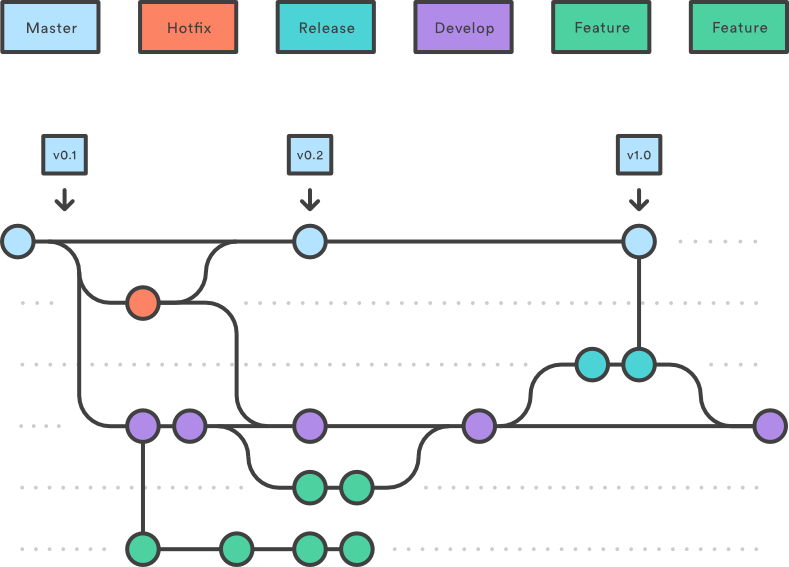
\includegraphics[width=0.7\linewidth]{imagens/gitflow.png}
	\caption{Exemplo de como \emph{GitFlow} funciona, exibindo os diversos \emph{branches} da metodologia.}
\end{figure}


%%%%%%%%%%%%%%%%%%%%%%%%%%%%%%%%%%%%%%%%%%%%%%%%%%%%%%%%%%%%%%%%%%%%%%%%%%%%%%%%%%%%%%%%%
\chapter{A Empresa e o Negócio}
%TODO Aqui precisamos falar sobre o historico e atividade da empresa (aka quem é o cara por trás da empresa, já que ela ainda não existe), o mercado, a concorrencia e escalabilidade do negocio. Boa parte disso aparece no Canvas mas nem tudo, então tem que ficar de olho

%TODO: corrigir TODAS as referências a "eu" (prim. pessoa do singular) para "nós", de acordo com a conversa com o Carlos

%%%%%%%%%%%%%%%%%%%%%%%%%%%%%%%%%%%%%%%%%%%%%%%%%%%%%%%%%%%%%%%%%%%%%%%%%%%%%%%%%%%%%%%%%
\section{Histórico}
A ideia originária para este projeto foi alimentada por alguns amigos do meio acadêmico e se desenvolveu para um sistema mais complexo e diferente. Foi decido transformar a ideia numa Startup\footnotemark{} e, a partir daí, iniciamos pesquisas na área, para entender melhor o funcionamento de empresas nesse formato e como seguir com um projeto nesse sentido.
\footnotetext{``Uma organização de formato temporário voltada para a busca de um modelo de negócios repetível e escalável''\cite{whats-startup}\cite{manual-startup}}

Durante o período de planejamento e execução do projeto, participei de diversas palestras, workshops\cite{workshop-startup} e eventos de networking, onde fiz contatos e conheci pessoas que puderam contribuir positivamente para as ideias do projeto. Em especial, durante o final do semestre 2015.1, participei da competição Sua Ideia Na Prática (SINP), organizada pela Ideation Brasil\cite{sinp-2015.1} -- uma organização voltada para o fomento do empreendedorismo universitário. Lá, entrei em contato com duas pessoas que tinham um projeto de fundo similar; unimos esforços e ganhamos o segundo lugar com nosso projeto. Durante o processo do evento, as ideias amadureceram e ganharam uma definição mais concreta, que é descrita neste documento. Como prêmio, recebemos uma consultoria jurídica e sessões com dois mentores nacionais, além de acesso a cursos da Endeavor.


%%%%%%%%%%%%%%%%%%%%%%%%%%%%%%%%%%%%%%%%%%%%%%%%%%%%%%%%%%%%%%%%%%%%%%%%%%%%%%%%%%%%%%%%%
\section{Descrição do mercado de eventos}
O mercado em que desejamos atuar pode ser dividido em duas macro-categorias, consideradas a partir do objetivo-fim de sua(s) atividade(s). Nesta divisão, o tamanho do público presente não é relevante. %TODO: buscar referências sobre os tipos de eventos

\begin{description}
	\item[Entretenimento e cultura em geral]
	Este grupo engloba atividades diversas, como: espetáculos teatrais, performáticos ou musicais; eventos beneficentes e de arrecadação de fundos; atividades esportivas, sejam competitivas ou recreativas. Estes eventos normalmente tem entrada controlada e paga, apesar de muitos (especialmente os beneficentes) também serem gratuitos, e algumas vezes, de entrada livre. Eles tendem a ter uma programação única e de interesse geral, apesar de alguns eventos musicais serem compostos de diversos palcos, cada um com atividades diferenciadas. Há também eventos mistos, compostos por atividades culturais e sociais.

	\item[Compartilhamento e construção de conhecimento]
	Aqui ficam categorizados eventos cujo objetivo é transmitir, divulgar e/ou debater novas informações dentro de um tópico, seja ele amplo ou específico. São representados por este grupo atividades de cunho tecnológico, científico, comercial, corporativo ou religioso. Em geral, as reuniões possuem uma programação mais elaborada, podendo ser composta por atividades simultâneas, que podem ser reunidas em torno de interesses distintos dentro do campo abordado. Podem ser pagos ou gratuitos, mas, em geral, possuem entrada controlada. De todos os eventos, deste e do outro grupo, os únicos que normalmente não possuem ampla divulgação são os corporativos -- por definição, estes são de interesse somente dos participantes de uma empresa ou entidade específica, e portanto recebem somente divulgação interna.
\end{description}

A partir desta divisão, podemos indicar o segundo grupo como sendo o foco inicial deste projeto.

Por um lado, o mercado do primeiro grupamento se encontra saturado de empresas oferecendo serviços como venda de ingressos, controle de bilheteria e atividades similares. É um mercado que movimenta mais de 70 bilhões ao ano somente no Brasil\cite{pegn-mercado-eventos}, e portanto, foi abocanhado por diversas companhias, algumas já consolidadas no setor, e outras mais novas, tentando ter sua fatia usando recursos inovadores.\\
Nestes eventos a programação, quando é diversificada, é facilmente assimilada pelos participantes, se necessário. Há também eventos com programação diversa e que se expande por vários dias. Num momento futuro, para expansão do projeto, planejamos também oferecer serviços que atendam esse tipo de público.

Por outro lado, para os outros eventos (de foco acadêmico, técnico ou profissional) há algumas empresas que fornecem serviços de organização e gerenciamento, mas, em geral, é um mercado com menor diversificação de ofertas. Há também uma necessidade maior de divulgação das atividades no congresso, visto que, diversas vezes, somente parte do público presente terá interesse no que será ministrado ou discutido em determinado momento.\\
Em eventos maiores ocorrem, com frequência, grupos distintos de discussões simultaneamente, o que também demanda que os participantes estejam informados dos assuntos e a localização das atividades. A necessidade de uma ferramenta mais eficiente de networking, se aproveitando das novas tecnologias móveis, também foi pauta frequente nas conversas com participantes.

O foco inicial deste projeto é o último grupo, a partir das necessidades citadas acima. As tarefas de comunicação e divulgação do evento aos interessados é tradicionalmente feita a partir de publicações em mídia especializada ou na internet; dentro dos eventos, ocorre a partir de panfletos, quadros informativos e mídia impressa em geral. Nosso objetivo é transformar os eventos em atividades mais interativas, dinâmicas e coesas, evitando os problemas comuns acarretados pela desinformação, como:

\begin{itemize}[itemsep=-1ex]
	\item desconhecimento da existência de eventos de menor porte, ou dificuldade de entrada do participante em novos mercados a partir dos eventos;
	\item atrasos e desencontros na programação;
	\item perda de atividades relevantes para o participante;
	\item problemas em localizar trabalhos e atividades de interesse;
	\item dificuldade em fazer \emph{networking}, reencontrando colegas ou fazendo novos contatos;
	\item complicações para encontrar locais agradáveis para alimentação durante o evento, e atividades de lazer antes e/ou após o mesmo, bem como de serviços de hotelaria além daqueles recomendados ou que fizeram parceria com a organização;
	\item desencontros quanto à distribuição e lotes dos ingressos, aumentando o custo de participação -- culminando até mesmo na desistência de alguns interessados.
\end{itemize}

\subsection{Os tipos de eventos-alvo} \label{sec:eventos}
De acordo com as atividades de divulgação de conhecimento, conforme citadas acima, há algumas dinâmicas distintas de eventos, que possuem objetivos diferentes e trabalham em torno destes. Os tipos mais comuns de eventos são\cite{tipos-manager}\cite{tipos-parlante}\cite{dicionario}\cite{dicas-feira-de-negocios}:

\begin{description}
	\item[Congresso] Tem objetivos e atividades mais diversificadas, visando ao debate de assuntos de um segmento específico, com atualização de conceitos do mercado, bem como exposição e divulgação de novidades. Normalmente é organizado por entidades associativas de foro nacional, regional ou internacional, e o público-alvo é o grupo de participantes destas entidades -- sendo, portanto, composto por pessoas com conhecimento dos temas. Possui uma programação diversa, normalmente sendo composto por mesas-redondas, conferências, simpósios, palestras, painéis, cursos e workshops. É interessante para manter e criar novos contatos, e se atualizar sobre o que ocorre no setor. Pela variedade e quantidade de atividades, estes duram de alguns dias a várias semanas, consumindo de 4 a 8 horas por dia.
	
	\item[Conferência] Uma reunião informativa composta por palestras formais. As atividades consistem de exposições de resultados por autoridades no assunto, e os questionamentos do auditório ocorrem somente no final, normalmente por escrito. O público já está familiarizado com o tópico do evento, e tem como objetivo a expansão ou atualização dos conhecimentos que já possuem. Também envolve networking, que pode gerar bons frutos, visto que os participantes em geral tem mais conhecimento sobre o tema abordado. %todo: pesquisar na internet a programacao de conferencias famosas e conferir se bate com o que ta escrito aqui
							
	\item[Convenção] Normalmente é promovida por entidades corporativas ou políticas. O maior objetivo das convenções é a integração e networking entre as pessoas daquela organização, gerando estímulos coletivos à interação do público. São apresentados temas diversos, mas sempre relacionados àquele grupo, levando os participantes a entender melhor o trabalho desenvolvido, e para que estes possam agir melhor em favor da instituição no futuro.
	
	\item[Seminário] O objetivo deste é a exposição de novos conceitos para um público interessado, mas menos informado no tema. Tende a ser mais parcial que os outros pois não há elementos de discussão dos tópicos abordados, e a fonte de informação normalmente é única -- o orador ou expositor do seminário, que usualmente é um expert no ramo. A atividade também pode ser presidida por mais de uma pessoa, num caso em que ambas as personalidades são complementares no assunto abordado. A programação de seminários normalmente é composta por uma ou algumas palestras, nesses moldes.
					
	\item[Simpósio] Um evento ou atividade aberta, objetivando o intercâmbio de informações e pontos de vista. A partir de um tema ou tópico específico, são desenvolvidos questionamentos e discussões entre os expositores e os próprios participantes, apresentando aspectos diferentes sobre o assunto -- que geralmente é científico e não é um amplo consenso no mercado. %todo ficou meio vago. Qual é a programaçao de um simposio e como eles sao englobados em eventos maiores (sao)?
	
	\item[Fórum] Tipo de evento no qual há a participação de um público numeroso, com programação mais abrangente e diversificada. A ideia é sensibilizar a opinião publica ou divulgar ao público assuntos de interesse geral, seja de setores específicos, da economia, ou sobre temas sociais ou políticos. Possui atividades mais gerais e abertas, para atrair e educar todo espectro de público.
	
	\item[Feira Comercial] Um tipo de exposição com foco em criação de novos contatos, descoberta de novos fornecedores e vendas. O principal elemento das feiras são os \emph{stands} das companhias participantes, que expõe seu rol de produtos e os novos lançamentos para o mercado. Em torno desses lançamentos eventualmente podem ocorrer apresentações com horário determinado, para que o público interessado venha a conhecer mais a fundo os detalhes dos produtos ou técnicas. Estas atividades comerciais também podem acontecer em menor escala, ou mescladas, na grade de programação de congressos -- demonstrando, por exemplo, novos produtos e tecnologias da área médica, que são de interesse dos profissionais presentes.
\end{description}

\subsubsection*{Eventos universitários ou técnicos}

Além dos diversos eventos de entretenimento e interação estudantil que acontecem todos os semestres nas instituições de ensino, há uma gama de eventos para graduandos e graduados dentro das universidades brasileiras. O foco vai desde o fomento à pesquisa ou empreendedorismo até atividades de cunho mais educativo, como versões reduzidas e mais leves dos congressos nacionais.

Para o público mais técnico ou profissionais de forma geral, alguns destes eventos também se aplicam, como os Encontros Regionais e Ciclos de Palestras. Assim como congressos, conferências e outros citados anteriormente, em geral estes são organizados por entidades de classe ou grupos independentes de indivíduos do ramo.

\begin{description}
	\item[Jornada de Iniciação Científica] Evento obrigatório para os alunos participantes de programas de Iniciação Científica (IC), que ocorre separadamente para cada curso da instituição. É similar à apresentação de resultados de pesquisa em congressos, onde há a opção de divulgar os resultados -- parciais ou finais -- em pôsteres ou apresentações. No caso do pôster, o estudante expõe e deve estar disponível no decorrer de um dia específico (há um rodízio de trabalhos) para perguntas de pessoas interessadas e, posteriormente, da comissão julgadora. Quando ele opta pela apresentação, há um \emph{slot} de tempo em que ele estará apresentando os resultados por meio oral e visual para uma plateia, composta também pela banca de jurados. Há uma premiação final dos trabalhos mais bem apresentados, inovadores, e afins. A decisão entre os tipos de divulgação varia entre cursos: pode ficar nas mãos do grupo de alunos ou dos coordenadores. Há a participação ocasional de curiosos de outros cursos e também de familiares dos alunos.
			
	\item[Encontro de Empresas Juniores] Os Encontros de EJ's costumam integrar grupos de empreendedorismo de uma instituição ou região específica, unindo as diversas especialidades. O evento funciona de forma similar a um congresso, com palestras e mesas-redondas em torno do assunto e workshops. O networking entre as empresas normalmente se dá durante os intervalos e refeições (bem pontuadas na programação diária\cite{enej15}), ou nos workshops, que são muitas vezes voltados para esse fim.

	\item[``Semana'' ou Encontro Regional] Um evento mais geral, que engloba diversas atividades para promoção da formação acadêmica dos participantes. Também é temática por curso. Em geral envolve diversas palestras no decorrer da programação; alguns cursos e workshops para fomentar a especialização em assuntos mais profundos; mesas-redondas para desenvolver tópicos mais complexos. Além disso, alguns currículos também envolvem saídas de campo, para experimentos e atividades práticas. As ``semanas'' também podem envolver diversos cursos similares, gerando atividades multidisciplinares e integrando estudantes de profissões afins.\\
	A diferença entre estes eventos e os Encontros Regionais se dá na participação: o último inclui diversas instituições de uma área geográfica específica, normalmente delimitada por um órgão nacional ou regional, e promove a troca entre estudantes que muitas vezes possuem experiências de ensino distintas.
	
	\item[Ciclo de palestras] Grupo de apresentações de cases e palestras, que não costuma tomar um dia inteiro, mas pode durar alguns dias. Normalmente gira em torno de um assunto mais específico dentro de um curso, ou pode englobar tópicos mais gerais e multidisciplinares, e integrar cursos distintos. Ocasionalmente também pode incluir workshops na programação.
		
	\item[Seminário] Semelhantes aos seminários comuns, mas voltados para um público mais iniciante.
\end{description}

\subsection{Atividades mais comuns}
Os eventos descritos acima, por vezes, são compostos por diferentes atividades. Em específico, simpósios, seminários e às vezes conferências também podem estar englobados em eventos de maior porte, como grandes conferências, congressos ou fóruns. Além destes, seguem aqui os componentes mais comuns dos eventos:
\begin{description}
	\item[Palestra] Apresentação por alguém mais inteirado num assunto a um público que tem interesse em se aprofundar no tópico. Pode ter diversos objetivos, como atualização curricular, discriminação de resultados, descrição de casos de sucesso, fins motivacionais, dentre outros. Dependendo da informalidade da atividade, questionamentos podem ser feitos durante -- de modo a não perder o foco em determinado tópico -- ou ao final -- para que o palestrante não perca seu próprio foco. Tende a durar cerca de uma hora, podendo se alongar. 

	\item[Mesa-redonda] Uma reunião presidida por um coordenador, que organiza e fomenta uma discussão sobre determinado assunto. Há uma apresentação inicial de pontos por cada um dos expositores (que podem ou não ser especialistas da área), e depois acontece um debate sobre os tópicos -- que, em geral, não são consolidados e levantam questionamentos --, em busca de algum tipo de deliberação. Auxilia os expectadores a se manterem informados e pensantes sobre o tema, de modo a gerar mais conhecimento e melhor entendimento sobre o que ocorre. Da mesa-redonda derivou o simpósio, que é uma versão mais ampla dessa atividade, e por vezes, mais extensa.

	\item[Painel de debates] Outro tipo de atividade similar à mesa-redonda. O foco maior é na discussão, pressupondo expectadores com mais conhecimento sobre o tema apresentado. A conversa tende a ser de mais alto nível, pois os participantes são especialistas, buscando gerar maior entendimento sobre os tópicos abordados.

	\item[Briefing/Keynote] Um tipo de palestra dada por alguém de renome na área, com o objetivo de introduzir algum assunto específico mais avançado, ou aprofundar as discussões que já aconteceram. Tende a acompanhar uma conferência, permitindo aos participantes obter maior entendimento do que será ou foi abordado nela.

	\item[Curso] Detalhamento de determinado assunto ou conjunto de assuntos com o objetivo de treinamento. Normalmente é ministrado por uma ou mais pessoas de formação acadêmica, e centrado na teoria -- apesar de também poder conter partes práticas. O público principal é composto por pessoas de pouco ou nenhum entendimento do tema, apesar de também existirem cursos de especialização, cujo foco é aprimorar os conhecimentos já existentes.

	\item[Workshop] Similar ao curso, mas tem um funcionamento mais focado na prática. É mais dinâmico e interativo, levando os participantes a assimilar os conteúdos por meio de discussões e atividades práticas. Muitas vezes também é parte de conferências, objetivando fixar melhor algum conteúdo apresentado na mesma.
\end{description}

%%%%%%%%%%%%%%%%%%%%%%%%%%%%%%%%%%%%%%%%%%%%%%%%%%%%%%%%%%%%%%%%%%%%%%%%%%%%%%%%%%%%%%%%%

\section{A modelagem de negócios da Lean Startup} \label{sec:modelagem-negocios}

Nesta seção do documento descreveremos muitos conceitos que são hipotéticos, relacionados a um projeto ainda em fase de concretização de ideias. Todos estes conceitos precisam ser confirmados por meio de entrevistas com os usuários ou pesquisas de mercado.\\
%Para facilitar a identificação, usaremos um marcador de Hipótese \hip{} ou de Confirmação \conf{} no início de cada afirmação relevante: o primeiro para aquelas que não foram testadas, e o segundo para as quais já verificamos serem procedentes -- aqueles que foram invalidados não estão incluídos aqui.

%%%%%%%%%%%%%%%%%%%%%%%%%%%%%%%%%%%%%%%%%%%%%%%%%%%%%%%%%%%%%%%%%%%%%%%%%%%%%%%%%%%%%%%%%

\subsection{\emph{Mapa de Empatia} - \emph{Personas} de nossos clientes e usuários}
O Mapa de Empatia\cite{mapa-de-empatia} é um diagrama simplificado que otimiza a identificação dos diferentes tipos de usuários e clientes. Seu principal conceito é a divisão de características comuns de seres humanos em diferentes blocos. Isto facilita a identificação de similaridades entre as pessoas que desejamos atender, e possibilita o desenvolvimento de um produto mais centrado no usuário. Tendo mais conhecimento sobre o tipo de pessoa que imaginamos resolver seu problema, podemos ir a campo encontrá-las e conversar sobre seus anseios e vontades, de forma que possamos entender exatamente como elas são e se o problema que identificamos existe de fato no mundo real.

Será possível notar, o tempo todo, como o conceito da \emph{Lean Startup} tem sempre como foco principal o(s) cliente(s) final(is): o objetivo é gerar algo que seja desejável e onde possa-se ouvir ``gostei! quero comprar agora!'', evitando o problema recorrente de se ter uma ideia mas não ter clientes para ela.

A \emph{persona}\footnotemark que descrevemos no diagrama \ref{diag:empatia} é uma estudante jovem, insegura e pouco preparada para o mercado. Suas características representam a união de sentimentos que temos e já tivemos em nossas carreiras, bem como impressões que coletamos ao conversarmos com outros universitários. Durante estas conversas, identificamos os principais ``pontos de dor'' neste tipo de usuário, quando falamos sobre o tópico ``eventos'':
\footnotetext{Personagem genérico com características em comum; a personificação de um grupo social}

\begin{itemize}[itemsep=-1ex]
	\item \iffalse\conf{}\fi a importância que os diversos eventos, dentro e fora da sua universidade, tem para sua formação extra-curricular;
	\item \iffalse\conf{}\fi o incentivo que alguns professores dão para a participação em atividades práticas, de campo ou de integração;
	\item \iffalse\conf{}\fi como algumas oportunidades foram perdidas por ineficiência de comunicação -- seja por terem perdido um anúncio em especial na instituição ou não terem contato com ``a pessoa certa'', que indicou determinado evento para um amigo mas não para ela, por exemplo.
\end{itemize}

\begin{figure}[!h]
	\centering
	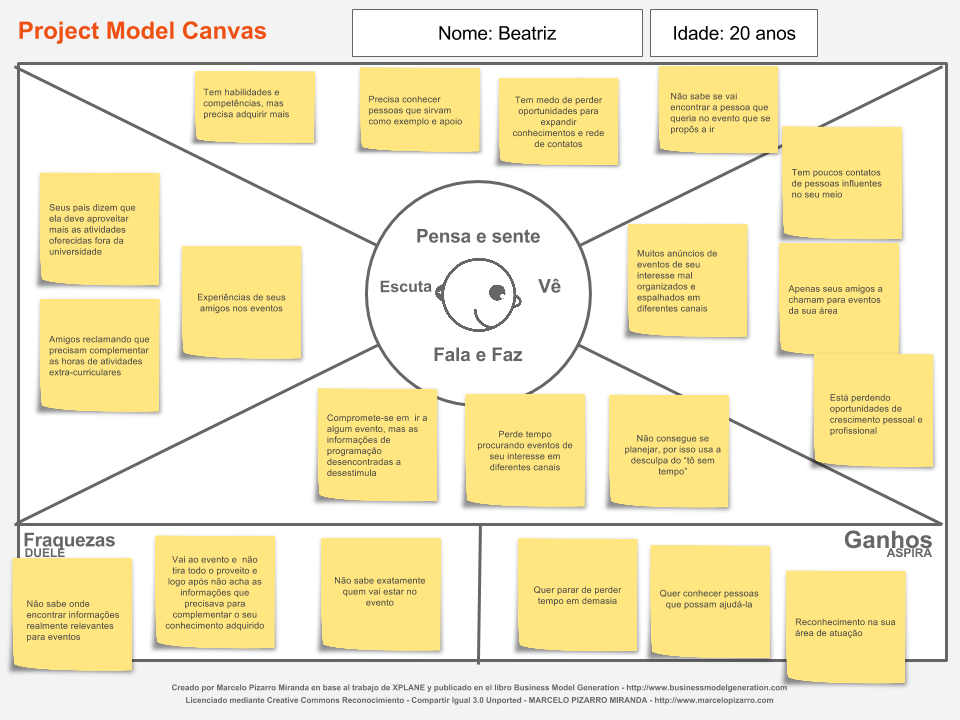
\includegraphics[width=1\linewidth]{diagramas/mapa-de-empatia.png}
	\caption{Mapa de Empatia de estudante. 1/jul/2015}
	\label{diag:empatia}
\end{figure}

%%%%%%%%%%%%%%%%%%%%%%%%%%%%%%%%%%%%%%%%%%%%%%%%%%%%%%%%%%%%%%%%%%%%%%%%%%%%%%%%%%%%%%%%%

\subsection{\emph{Árvore de problemas} - Visualização das principais dores}
De forma a entender melhor o outro lado do problema, a partir de um \emph{brainstorm} desenvolvemos outro diagrama, chamado de Árvore de Problemas. Ele é formado por um bloco central, que indica o problema básico que estamos investigando, e ramificações de causas e consequências do mesmo.\cite{arvore-de-problemas-portal-educacao}

Muitas vezes o que nos é relatado é só a ``ponta do iceberg'', a parte mais superficial da questão. Para resolvê-la, no entanto, pode ser necessário ir mais a fundo de modo a evitar que o problema ocorra novamente. Com a Árvore, é possível entender de forma clara quais são as origens do \emph{pain point} do cliente.

O desenvolvimento da Árvore de Problemas é um exercício mental de abstração e pensamento fora da caixa, que nos força à introspecção enquanto tentamos desvendar os problemas que o cliente citou durante as entrevistas. Uma das técnicas para desenvolvê-la é a dos Cinco Porquês\cite{five-whys} (ou três\cite{three-whys}\cite{three-whys-semler}, dependendo do autor e do nível de especificação que desejamos), que visa se aprofundar numa questão inicial para chegar às suas raízes.

\begin{citacao}
	Quando confrontado com um problema, você já tentou alguma vez parar e perguntar ``por que'' cinco vezes? É difícil de fazer mesmo que soe fácil. Por exemplo, suponha que uma máquina tenha parado de funcionar:
	
		1. Por que a máquina parou? \emph{Houve uma sobrecarga e o fusível estourou.}\\
		2. Por que houve a sobrecarga? \emph{O rolamento não estava lubrificado o suficiente.}\\
		3. E por que não havia lubrificação suficiente? \emph{A bomba de lubrificante não estava bombeando o suficiente.}\\
		4. Por que não bombeava o suficiente? \emph{O eixo da bomba estava gasto e chacoalhando.}\\
		5. E por que ele estava gasto assim? \emph{Não havia nenhum filtro na bomba e partículas de metal entraram.}
		
	Repetir ``por que'' cinco vezes, dessa forma, pode nos ajudar a desencavar a raiz do problema e corrigi-lo. Se este procedimento não fosse tomado, alguém poderia simplesmente ter trocado o fusível ou o eixo da bomba. Nesse caso, o problema aconteceria novamente em alguns meses. O sistema de produção da Toyota foi construído a partir da prática e evolução deste método científico. Ao perguntar e responder o porquê cinco vezes, nós podemos chegar à real causa do problema, que muitas vezes está escondida embaixo de sintomas mais óbvios.
	
	{\raggedright (\citetext{five-whys} Tradução nossa.)}
\end{citacao}

\begin{citacao}
	\textbf{O jeito ``por que''}
	
	O segredo? Se nós temos uma estratégia cardinal que forma a pedra de fundação de todas as nossas [da Semler] práticas, pode ser isso:\\
	Perguntar por que.\\
	Perguntar isso todas as vezes, perguntar isso qualquer dia, todos os dias, e sempre perguntar isso três vezes seguidas.
	
	Isso não vem naturalmente. Pessoas estão condicionadas a evitar perguntar demais. Primeiro, isso pode soar rude. Segundo, pode ser perigoso, implicando que somos ignorantes ou desinformados. Terceiro, significa que tudo que nós pensamos que sabemos pode se tornar incorreto ou incompleto. [...] Isso significa colocar de lado todas as respostas rotineiras e pacificadoras [\emph{rote and pat answers}] [...], aquele estado da mente onde as ideias se tornaram tão endurecidas que elas não tem mais uso nenhum. [...] E uma empresa precisa ser flexível o suficiente para ouvir estas respostas. Esses hábitos são a chave para a longevidade, crescimento, e lucro.
	
	{\raggedright (\citetext{three-whys-semler} Tradução nossa.)}
\end{citacao}


\begin{figure}[!h]
	\centering
	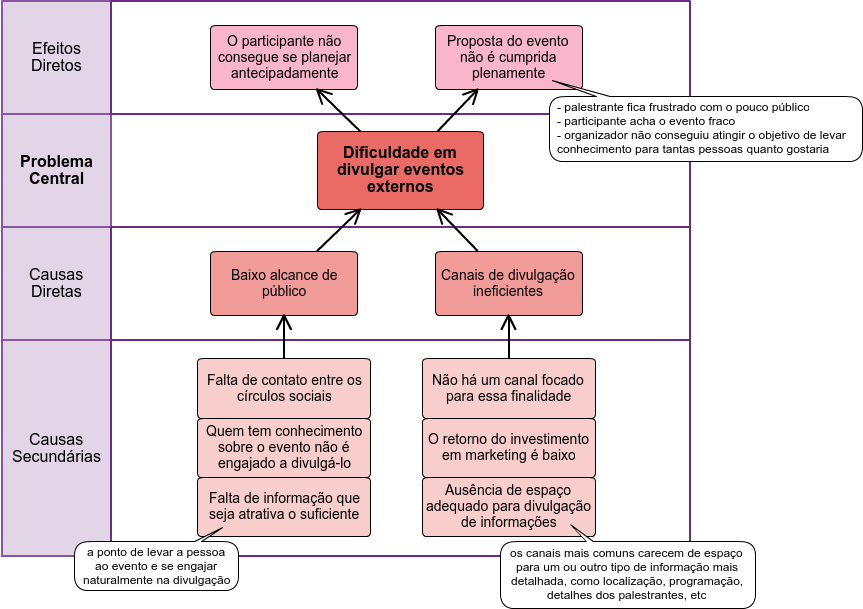
\includegraphics[width=1\linewidth]{diagramas/arvore-problemas-divulgacao.png}
	\caption{Árvore de Problemas - Divulgação Externa. 3/jul/2015}
	\label{diag:arvore}
\end{figure}

O problema que desenvolvemos no diagrama \ref{diag:arvore} é referente à dificuldade de divulgação de eventos abertos ao público além da própria organização -- aqui chamados de ``eventos externos'', em contraste com eventos internos da organização, em que todos os participantes recebem convites expressamente. Esta situação é causada pelo problema em alcançar o público-alvo e por usar de canais ineficientes. Por sua vez, ela leva a uma falha na proposta do evento, seja devido à frustração do palestrante ou do público, por dar a impressão de que o evento foi ``fraco''; a frustração do participante pode ser tomada como uma consequência à parte, visto que divulgação ineficiente, atrasada ou com informações desencontradas pode levá-lo a problemas de planejamento para participar das atividades.

%%%%%%%%%%%%%%%%%%%%%%%%%%%%%%%%%%%%%%%%%%%%%%%%%%%%%%%%%%%%%%%%%%%%%%%%%%%%%%%%%%%%%%%%%

\subsection{\emph{Lean Canvas} - Um modelo de negócios iterável}

\begin{figure}[!bp]
	\centering
	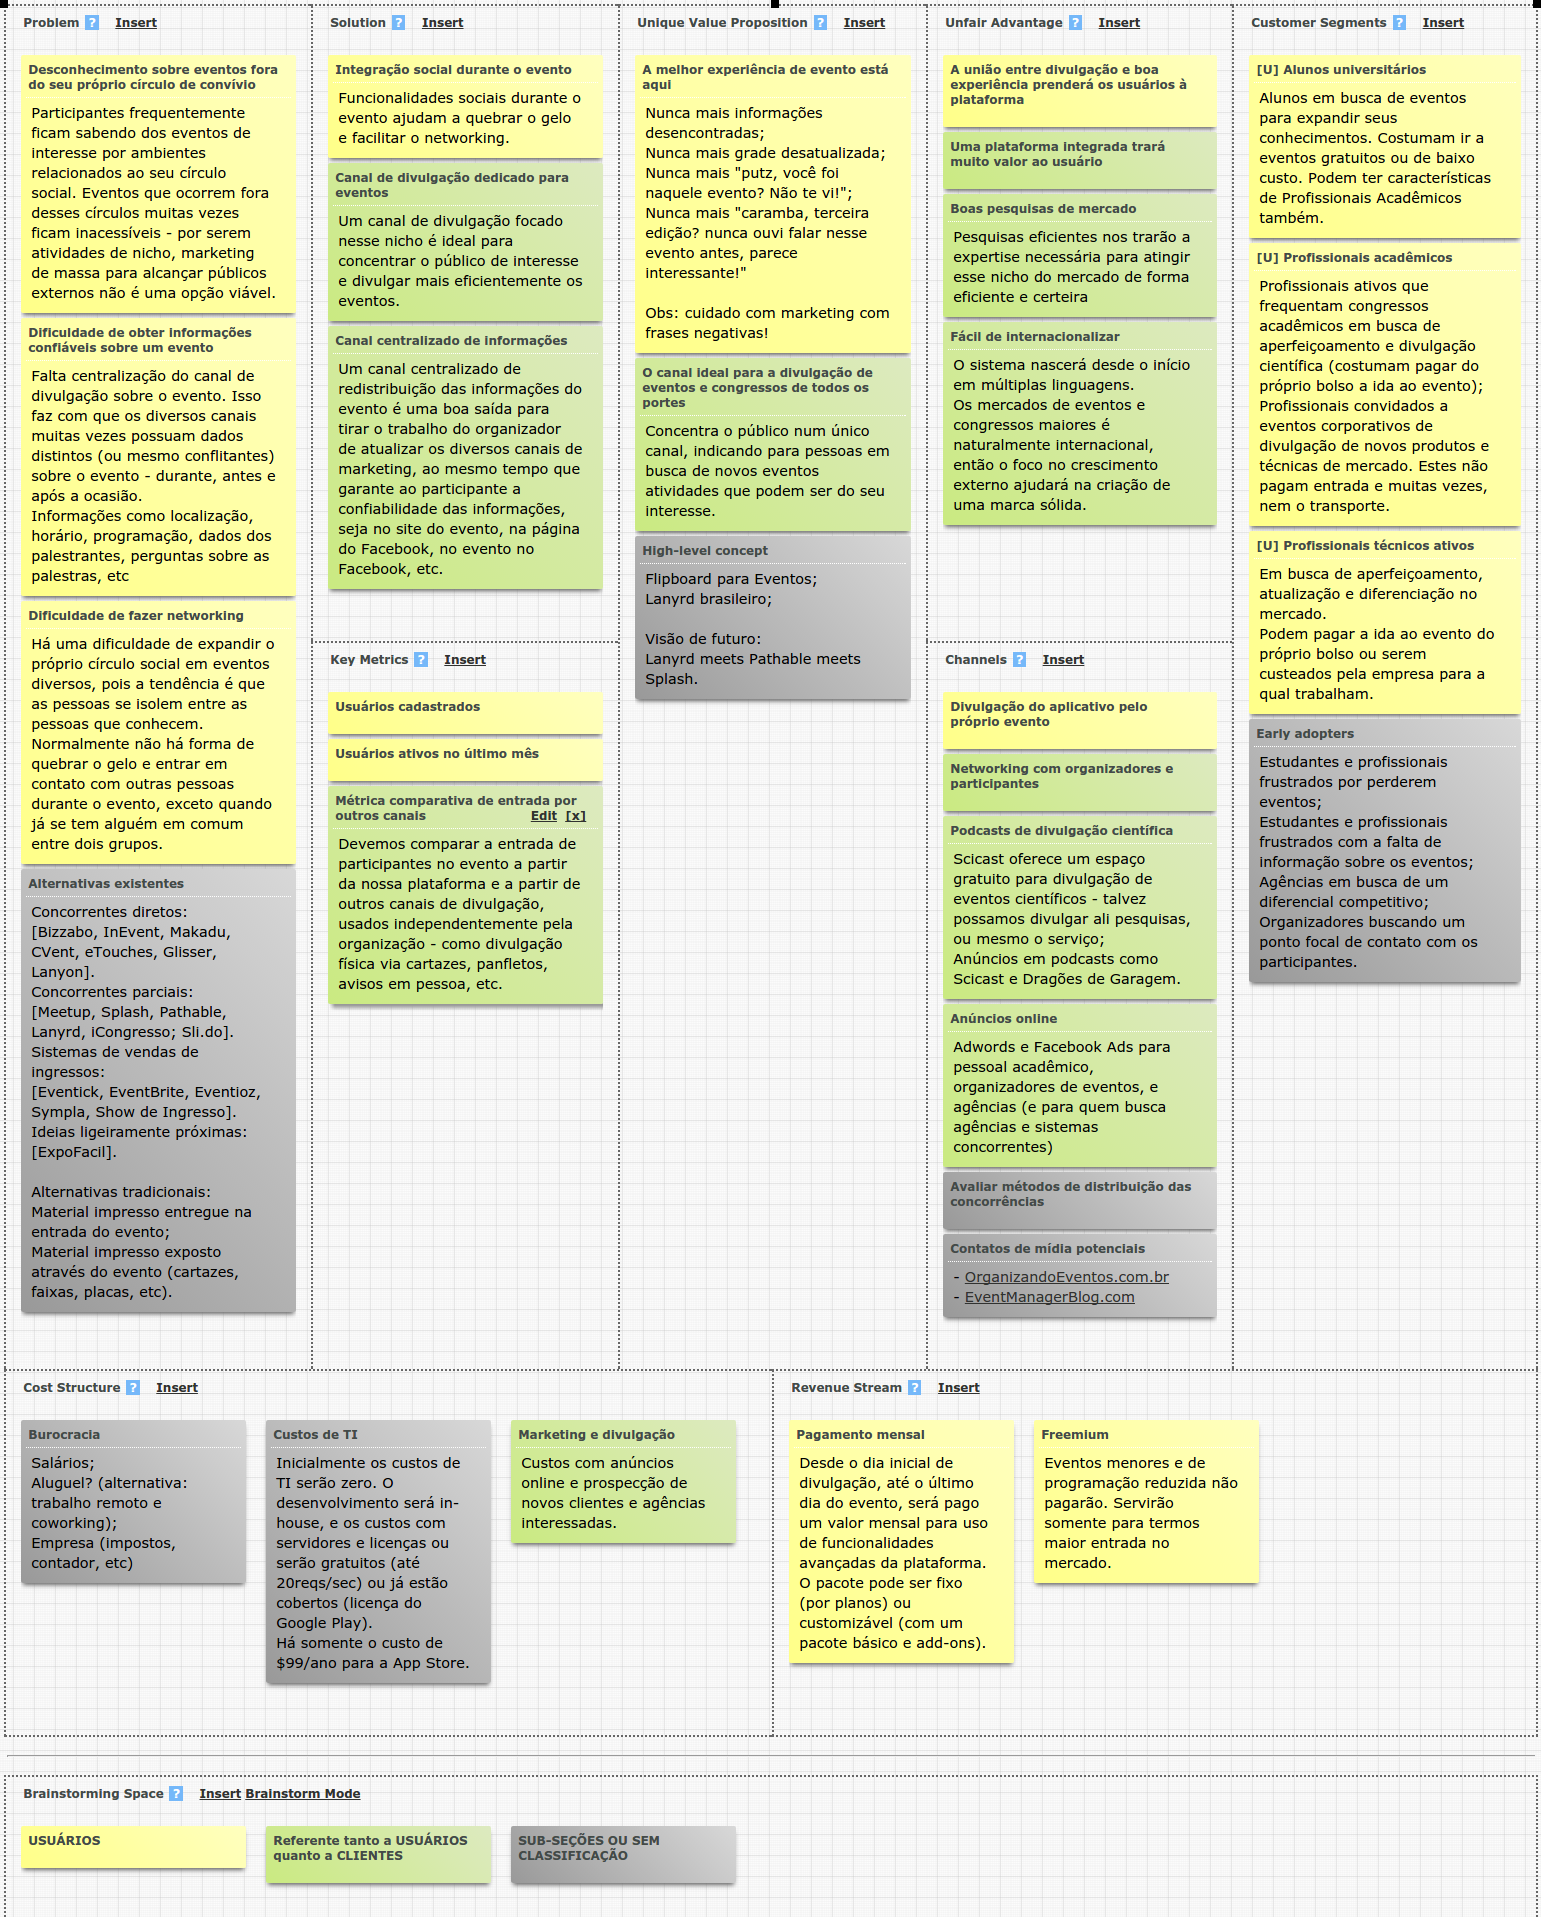
\includegraphics[width=1\linewidth]{imagens/canvas-usuarios.png}
	\caption{Lean Canvas do usuário. 16/ago/2015}
	%todo: avaliar legibilidade do diagrama quando impresso em A4
\end{figure}

Segundo \citeauthor{manual-startup} (p.~83), frequentemente, em equipes e empresas novas, há confusão de informação e dificuldade de entendimento de qual é exatamente o modelo de negócios que será utilizado. Portanto, foi decidido usar o \emph{Lean Canvas} para ilustrar de forma rápida e eficiente os principais pontos deste projeto.

Originalmente, Alex Osterwalder criou o \emph{Business Model Canvas}, buscando resumir todos os lados de uma empresa num quadro de nove caixas, de forma que todos eles pudessem ser confrontados de um jeito rápido e por qualquer pessoa da companhia, e facilmente alterado e  corrigido. Posteriormente, Ash Maurya criou o \emph{Lean Canvas}, se baseando no original mas alterando algumas das caixas, objetivando focar nas partes mais importantes (arriscadas) e mutáveis de uma startup.\cite{why-lean-canvas}

Ainda de acordo com \citeauthor{lean-canvas}, é importante criar uma versão do \emph{canvas} para cada grupo de clientes da companhia. No nosso caso, com um produto multifacetado, por um lado precisaremos servir e atrair os organizadores de eventos, que pagarão pelo serviço e desejam melhorar a comunicação com seus congressistas; por outro, os participantes precisam se sentir confortáveis dentro da plataforma e com vontade de saber mais sobre ela nas divulgações, interessados em utilizá-la, e vendo proveito no decorrer do uso. Essa dualidade reflete os dois lados do sistema, onde precisamos satisfazer tipos distintos de \emph{personas}, com necessidades e objetivos diferentes. Portanto, o sistema terá dois \emph{canvas} que evoluirão em sintonia. No entanto, para o escopo deste projeto, focaremos nossos esforços no usuário final; os motivos serão esclarecidos oportunamente. %todo: verificar se foram esclarecidos!

Uma consequência da natureza mutante do \emph{canvas} é que ele dificilmente será ``gravado em pedra''; durante o trabalho na definição deste projeto, ideias novas surgirão e hipóteses serão criadas, aperfeiçoadas ou descartadas -- e a cada novo passo, os \emph{canvas} deverão ser atualizados. Nesta seção vamos exibir somente a versão atual do documento, e o histórico poderá ser conferido online, no endereço \mbox{\url{https://canvanizer.com/canvas/2MM3fHvw8Lo}}.

\iffalse
Também descreveremos em síntese os blocos adicionais do \emph{Business Model Canvas}. Estes não são tão mutáveis, mas também são dignos de uma discussão inicial, por fazerem parte da criação da companhia.
\fi

\subsubsection*{Bloco Zero: Pesquisa de mercado}
\label{sec:lean:mercado}
Ao descrever o processo de \textit{Customer Discovery} (Descoberta do Consumidor) no livro Manual da Startup\cite{manual-startup}, \citeauthoronline{manual-startup} sugerem criar um resumo inicial sobre o tamanho do mercado antes de iniciar as sínteses de cada parte do Business Model Canvas.

Inicialmente, precisamos considerar que o projeto é um sistema de duas saídas: por um lado, estaremos atendendo os organizadores de eventos, que objetivam se comunicar com seus participantes; por outro, estaremos atendendo os próprios participantes, que desejam obter as informações que os organizadores disponibilizarão sobre os eventos que os interessam. Portanto, é importante notar que, apesar do mercado ser um só, há dois tipos distintos de consumidores a se considerar neste ramo.

\textbf{Para os fins deste documento, estaremos considerando como ``clientes'' os organizadores de eventos, e ``usuários'' os participantes (os consumidores finais do sistema).}

Dito isso, nosso \underline{mercado disponível} é o segmento de eventos acadêmicos, científicos e técnicos.

Desse grupo, o \underline{mercado disponível para negócios} é o grupo de usuários que possuam um smartphone, tablet ou computador com conexão à Internet, conforme a \autoref{sec:tecnologias}. Além disso, inicialmente focaremos nos países lusófonos e anglófonos, com versões do sistema em português e inglês. O mercado disponível de clientes é definido pelos mesmos requisitos de linguagem, mas o requisito técnico passa a ser o uso confortável de um computador com Internet, visto que no início as atividades de atualização de informações são mais práticas de serem executadas num dispositivo como esse, dada a quantidade de informações que precisarão ser inseridas e analisadas.

Por fim, nosso \underline{mercado-alvo} será o grupo de organizadores que sentem dificuldade em divulgar e espalhar informações sobre seus eventos, ou, ainda, que desejem melhorar a comunicação com seus participantes, melhorando a fidelização e aumentando a venda de ingressos. Há também o grupo de congressistas, cujo alvo principal será aqueles que já se sentiram frustrados pela falta de informações ou confusos quanto às atividades de um evento; que tem interesse em descobrir novos eventos ou explorar novos mercados; ou que se sentem curiosos por forma mais eficiente e instantânea (móvel) de obter detalhes sobre o evento, tanto antes do mesmo quanto no instante.

%todo calcular estimativas numéricas dos mercados

É importante notar também que os nossos alvos iniciais serão o mercado de eventos tecnológicos open source, com os quais temos contato direto; e grupos de interesse científico universitários, onde executaremos pesquisas e trabalhos de divulgação iniciais.

\paragraph*{\iffalse\protect\hip{}\fi A partir da descrição do mercado, podemos tirar as seguintes hipóteses:}
\begin{description}[itemsep=-1ex]
	\item[Mercado] organizadores (\textit{clientes}) e participantes (\textit{usuários}) de eventos acadêmicos, científicos e técnicos.
	\item[Mercado disponível] clientes com computadores com acesso à Internet; usuários com computadores ou dispositivos móveis com acesso à Internet; ambos falantes de português ou inglês.
	\item[Mercado-alvo] clientes com dificuldade de divulgação ou que já experimentaram problemas na comunicação com os participantes; usuários com interesse direto ou indireto em informações mais eficientes sobre um evento específico, ou com interesse em descobrir novos eventos.
	\item[Mercado-alvo primário] eventos de tecnologia open source; eventos científicos de origem universitária.
\end{description}


\iffalse %todo: completar e adicionar de volta as seções sobre o Canvas e o Experiment Board
\subsubsection*{O \emph{Canvas} dos Usuários (congressistas)}

\paragraph*{1 - O Problema \emph{(Lean Canvas)}}
\begin{description}
\item[hip{} Dificuldade de organização e filtragem de atividades de interesse] 
O congressista tende a enfrentar dificuldades quando a grade de palestras é liberada. Inicialmente ele escolhe tópicos de interesse e tenta selecionar a parte da programação que mais lhe agrada. No entanto, é difícil transportar esse planejamento para o dia do evento. Isso normalmente é feito de memória, com anotações, ou às vezes com entradas no calendário do celular.\\
Além disso, é comum a distribuição de folhas com a programação do dia ou do evento inteiro; no entanto, é comum que esse material se perca ou danifique no decorrer do dia, seja em meio a tantos itens promocionais ou mesmo ao ser dobrado e colocado no bolso.

\item[\hip{} Dificuldade em acompanhar eventos novos e em andamento]
Não é incomum que os interessados demorem a saber dos eventos, apesar dos esforços de marketing empregados. Muitas vezes os ingressos são comprados em lotes avançados não pela dúvida em ir, mas pelo simples desconhecimento. Além disso, também acontece de o inscrito não conseguir acompanhar as novidades sobre sua participação, como divulgação de palestrantes, da grade de programação ou pequenas alterações na estrutura do congresso. Avisos de última hora, como informações sobre alimentação e documentos necessários, podem se perder nos dias que antecedem o evento.

\item[\hip{} Problemas em coletar informações para networking]
Um dos grandes objetivos de eventos técnicos e científicos é a concretização de novos laços profissionais. O mesmo se dá comumente em situações formais ou informais dentro dos eventos, como durante mesas-redondas e discussões em geral, nos coffee-breaks, refeições ou happy hours. No entanto, no final do evento às vezes é complexo manter o contato com os novos colegas, por causa do volume de cartões de visita trocados e a parca identificação dos mesmos, ou mesmo pela perda destes. Há também o caso em que os dados são perdidos ou anotados incorretamente, o que leva ao fracasso na tentativa de contato. Isso também ocorre com dados de contato dos palestrantes, que muitas vezes são divulgados somente nos slides apresentados.

\item[Outros problemas] Há também problemas de menor porte, mas que comumente afetam os congressistas, como os listados a seguir:
	\begin{itemize}[itemsep=-1ex]
		\item \hip{} Dificuldade e ineficiência na localização e estudo de trabalhos expostos no salão do congresso;
		\item \hip{} Morosidade e lentidão no processo de avaliação dos projetos apresentados;
		\item \hip{} Dificuldade em descobrir e localizar bons restaurantes para comer nos intervalos, que fiquem próximos ao local do evento. Há indicações da organização, mas por vezes os locais estão lotados ou não são do interesse do congressista. O mesmo pode ocorrer também com opções de hospedagem, ou pontos de interesse para visitação na cidade;
		\item \hip{} Por desconhecimento da região, o congressista às vezes enfrenta dificuldade para se locomover ao local do evento, já que não conhece os meios de transporte público locais;
		\item \hip{} Considerando a concentração de pessoas no mesmo local, é de se esperar que haja congestionamento nas redes Wi-Fi do evento, ou mesmo nas redes celulares no interior dos prédios. Decorrente disso, os congressistas ficam sem acesso à Internet, o que pode ocasionar dificuldade para obtenção de informações no site do evento ou em seus e-mails, por exemplo.
	\end{itemize}
\end{description}

\subparagraph*{Alternativas existentes}
\begin{description}
\item[\conf{} Bizzabo] Startup israelense que está entrando no mercado brasileiro, com direção de pessoas influentes no mercado de startups nacionais. O primeiro uso conhecido no país foi o CASE 2014, a conferência da Associação Brasileira de Startups. Mais detalhes sobre a empresa e seu sistema podem ser vistos na \autoref{sec:concorrencia:bizzabo} e na \autoref{sec:sistemas:bizzabo};

\item[\hip{} Aplicativos próprios] Alguns eventos possuem aplicativos próprios (\autoref{sec:sistemas:apps_privados}), que em geral são considerados pelos participantes como ineficientes, fracos, e com poucas funcionalidades -- e, eventualmente, nem são considerados funcionais;

\item[\hip{} Site do evento] Normalmente há informações divulgadas no site do evento. No entanto, estas dificilmente são úteis na data, pois nem sempre estão atualizadas e é comum a conexão falha no local. Detalhes na \autoref{sec:sistemas:divulgacao};

\item[\hip{} Comunicação impressa no local] Por fim, há diversas formas de sinalização gráfica, como panfletos, cadernos, cartazes e folhas com a programação, dados de localização interna, dentre outros. No entanto, estes materiais tendem a se deteriorar ou se perder com o decorrer do evento. Mais informações na \autoref{sec:sistemas:outros};

\item[\hip{} Sistemas paralelos] Há também empresas que não apresentam concorrência direta num primeiro momento, como sistemas de organização e gerenciamento de eventos, ou de venda de entradas (\autoref{sec:concorrencia:organizacao_venda} e seções \ref{sec:sistemas:gerenciamento} e \ref{sec:sistemas:venda}).
\end{description}

\paragraph*{2 - Segmentos de consumidores}
Os segmentos de usuários que pretendemos atingir são os seguintes:
\begin{description}
	\item[\hip{} Congressista de TI] Este usuário frequenta eventos que, em geral, possuem palestras, \emph{lightning talks}, às vezes workshops e keynotes. Também ocorrem exposições de patrocinadores. Estes eventos dificilmente (se é que) tem divulgação de pesquisas, mesas-redondas e outras atividades. Eles também não costumam durar mais de 2 ou 3 dias, e há muitos que duram um dia só.

	\item[\hip{} Congressista de Ciências] Este tipo de usuário costuma ir a eventos mais longos e com mais variedade de atividades. Eles possuem, comumente, menos aptidão tecnológica e dispositivos menos modernos são comuns também.

	\item[\hip{} Congressista de Humanas] Similar aos usuários de Ciências, mas com uma variedade um pouco diferente de atividades nos eventos, por muitas vezes tratarem de assuntos mais abstratos.
\end{description}

\subparagraph*{O usuário inicial - \emph{early adopter}, ou \emph{earlyvangelist}} ~\\
É essencial que possamos definir quem é o típico \emph{early adopter} do nosso produto. Um \emph{early adopter} é aquele usuário que se identifica muito com o problema que nos propomos a resolver, e percebe na nossa empresa a chance de ter aquilo solucionado. Este personagem é uma peça chave no desenvolvimento e no futuro do projeto. No início, ele auxilia com testes precisos e sugestões diversas, sendo um correspondente ideal dos anseios dos usuários, por vir diretamente do grupo deles. Por ser o usuário mais ferrenho, o \emph{early adopter} tende a ter necessidades mais amplas, trazendo a bordo novas ideias e a chance de cobrir cada vez melhor os requisitos dos usuários comuns também. Devido à sua avidez, eles também podem ser chamados de \emph{earlyvangelists}, pois quando percebem que o produto os satisfaz, ficam felizes em divulgar gratuitamente a seus canais sociais -- o que traz ao produto marketing sem custos, e do melhor tipo possível: a indicação direta. No longo prazo a tarefa de evangelização se mantém, enquanto suas necessidades devem continuar sendo ouvidas para que não percamos os usuários de vista e continuemos a atendê-los satisfatoriamente.

Dito isso, podemos identificar que um \emph{early adopter} típico do nosso produto será:

\begin{description}[itemsep=-1ex]
	\item[\hip{} Jovem, de de 18$\sim$30 anos] potencialmente mais conectado e ativo, física e socialmente, e com mais facilidade para utilizar tecnologia;
	\item[\conf{} Dono de um smartphone recente (não necessariamente de última geração)] não terá impasses em baixar, instalar e utilizar todas as funcionalidades do aplicativo;
	\item[\hip{} Da área de TI] há mais diversidade de eventos durante o ano, e menor variedade de atividades -- o que significa mais foco no que importa durante os passos iniciais do aplicativo;
	\item[\conf{} Morador de metrópoles] há maior concentração de eventos, tanto no mercado nacional quanto internacional; %todo: devemos focar mais no mercado nacional dada a concorrência do Bizzabo, ou focar em todos os mercados para gerar concorrência desde o princípio?
	\item[\conf{} Frequentador assíduo de eventos] que frequente eventos de médio/grande porte (pela variedade de conteúdos) pelo menos 2x ao ano, além de encontros mais informais de desenvolvedores e palestras.
\end{description} 
% descrever porque é importante saber quem é o early adopter e porque ele é importante para a startup, e daí descrever quem será o nosso

\paragraph*{3 - A Solução}

\paragraph*{4 - Proposta de valor} % O produto, benefícios e MVP
% Hipotese final: single, clear and compeling message that states why your product is different and worth buying

\paragraph*{5 - Canais de distribuição}
%uma das ideias pra divulgar o app é bme simples:
%divulgar entre os organizadores, e deixar q eles divulguem o app aos seus congressistas
%
%e outra é arrumar algum time de redes sociais, talvez contratar alguem ou um freelancer, e deixar ele tomando conta das redes
%de criar um blog, de postar no facebook, twitter, talvez fazer contato com organizações e eventos em geral vendendo a ideia tbm, pesquisando por aí eventos que existam e entrando em contato, sei lá... nao sei ainda
%
%eu acho que, inicialmente, aqui no brasil eu vou divulgar por conta propria
%com amigos e afins, fazendo as pesquisas nas universidades q conheço e q consiga contato
%e la pra fora vou colocar anuncios no google pra poder angariar pessoas que falem ingles pra rodar pesquisas na gringa tbm
%pq tem duas frentes né, quem paga e quem usa
%quem paga eu acho que a divulgação vai ser mais pelo boca-a-boca de quem já conhece, por anuncios no google, e por divulgacao minha mesmo
%quem usa acho q em parte vai ser pelo proprio evento, e talvez quando ja tiver tracking colocar anuncios no facebook e google tbm
%pq pra colocar usuario pra dentro eu preciso de eventos participando do app
%dai eu tendo um produto basico eu vou distribuir betas pros eventos q eu ficar sabendo (to anotando todos q eu descubro pelas newsletters que assino)
%pra poder ter massa de manobra
%e ai sim, tendo eventos, eu consigo divulgar pros usuarios e dizer "ei, os eventos mais interessantes e modernos tao aqui! vem ver, instala aí"
%e dps disso, tendo mais usuarios, eu consigo convencer mais organizadores a colocar seus eventos no app, e por ai vai

\subparagraph*{Relacionamento com o consumidor \emph{(Business Model Canvas)}}

\paragraph*{6 - Estrutura de custos}

\paragraph*{7 - Fonte de receita}

\paragraph*{8 - Principais métricas}

\paragraph*{9 - Atividades-chave \emph{(Business Model Canvas)}} % Hipóteses de mercado e diferenças competitivas

\subparagraph*{Vantagem de mercado}

\paragraph*{Recursos-chave \emph{(Business Model Canvas)}}

\paragraph*{Parceiros-chave \emph{(Business Model Canvas)}}

%%%%%%%%%%%%%%%%%%%%%%%%%%%%%%%%%%%%%%%%%%%%%%%%%%%%%%%%%%%%%%%%%%%%%%%%%%%%%%%%%%%%%%%%%


\subsection{\emph{Experiment Board} - Hipóteses a serem avaliadas}
Considerando que uma startup é baseada em hipóteses não testadas, é necessário que tenhamos um roteiro e uma forma padronizada de seleção e listagem de hipóteses. Estas, posteriormente, devem ser verificadas ou refutadas a partir de experimentos diversos, como pesquisas, entrevistas, ou análises.

\begin{citacao}
	%Customer development é um processo baseado em hipóteses para entender: quem são seus consumidores; quais problemas e necessidades eles tem; como eles se comportam atualmente; por quais soluções eles pagariam (mesmo que o produto ainda não esteja feito ou completo); como fornecer soluções de uma forma que combine com a forma que seus consumidores decidem, adquirem, compram e usam.
	
	Você provavelmente tem idéias e intuições sobre [todas essas hipóteses]. Vamos identificar o que elas realmente são: chutes. Vamos fazê-las soar um pouco melhor e chamá-las \emph{hipóteses}. Essas hipóteses podem ser sobre formar uma nova empresa, criar um novo produto, ou mesmo adicionar novas funcionalidades ou capacidades a um produto existente.
	
	\emph{Tudo que você faz durante [essa fase] é centrado em torno de testar hipóteses.}
	
	{\raggedright (\citetext{lean-customer-development} Cap. 1. Grifo do autor, tradução nossa.)}
\end{citacao}

Tendo isso em mente, decidimos usar o \emph{Experiment Board} (criado por uma empresa chamada \citeauthoronline{experiment-board-javelin}) para definir as hipóteses relevantes do nosso produto, e a melhor forma de testá-las. Muitas hipóteses são indicadas na descrição do Lean Canvas, posteriormente, mas aquelas descritas nesta seção são de cunho mais amplo, cobrindo um espectro mais diverso do projeto. Nosso objetivo é indicar as hipóteses gerais do sistema de uma forma que seja fácil de testar -- pois na maior parte das vezes, as ideias são tão grandes que é necessário fragmentá-las para torná-las testáveis\cite{experiment-board-post}.

O \emph{Experiment Board} funciona listando todos os tipos de Clientes, seus Problemas, possíveis Soluções e Riscos potenciais. Depois disso, cruzamos estes quatro elementos e formulamos uma hipótese. Devemos decidir o método de teste e o critério que definirá se a hipótese foi confirmada ou refutada. Ao final do teste, indicamos o resultado e o que foi aprendido com o teste. No caso de a hipótese ter sido refutada, seus elementos devem ser revistos e novos testes, feitos -- numa ação conhecida como ``pivotar'', onde os elementos principais são mantidos mas a direção da ideia é alterada, de forma a ter uma nova visão sobre a questão.

Usaremos neste projeto uma versão modificada do quadro, fornecida no Workshop de Criação de Startups do Circuito Startup\cite{workshop-startup}. As principais diferenças são: a remoção dos blocos de texto de ajuda; a quebra das áreas de Cliente e Problema em duas (o que nos facilita, visto que nosso mercado é multi-facetado [ver \autoref{sec:lean:mercado}]); e o fato de que a principal hipótese não deve possuir solução pronta -- por ser o principal motor do produto, a solução seria ele mesmo.

%todo adicionar aqui uma foto do experimental board mais preenchido

%todo listar aqui as hipóteses encontradas, métodos e critérios

\fi

%%%%%%%%%%%%%%%%%%%%%%%%%%%%%%%%%%%%%%%%%%%%%%%%%%%%%%%%%%%%%%%%%%%%%%%%%%%%%%%%%%%%%%%%%

\section{Concorrência}
Foi encontrada somente uma empresa que preste serviços diretamente relacionados ao espectro do mercado que pretendemos cobrir com nosso projeto: o Lanyrd. Ainda assim, o projeto parece estar num estado letárgico desde sua compra pela EventBrite, em 2013 (mais informações na \autoref{sec:concorrencia:lanyrd}).

Além deles, há alguns sistemas similares, mas com foco em outros mercados (\autoref{sec:concorrencia:outros-mercados}): Upcoming.org, focado em eventos artísticos e de nicho; Meetup, focado em encontros informais e sociais; All Events in City e outros, focados em eventos sociais em geral. Estes podem servir de exemplo e de fonte de ideias, mas não representam concorrência direta ao nosso projeto.

No mercado nacional não há concorrência real, visto que o único projeto similar existe somente em inglês -- fato tomado como negativo por alguns usuários dele entrevistados no Brasil. Dos sistemas listados, o único que possui versão em português -- Meetup -- foi citado em entrevistas ocasionais, mas com seu uso somente no campo de eventos mais intimistas e reduzidos (de 5 a 50 participantes).

Por fim, há outros tipos de sistemas no mercado de eventos, mas com outro propósito e que somente tangencia nossos objetivos: a venda de ingressos (\autoref{sec:concorrencia:venda}). Em especial, a Sympla, EventBrite e Eventick são dignos de nota, por serem os maiores \emph{players} no cenário nacional e internacional (nesse sub-grupo, o principal destaque é a EventBrite). A venda de entradas é considerada uma boa aposta no campo de monetização do projeto, mas por se tratar de um módulo com complexidades técnicas e burocráticas, pode ser alcançado inicialmente de forma mais simples a partir de parcerias com empresas como as citadas.

\subsection{Lanyrd} \label{sec:concorrencia:lanyrd}
Criado em 2010, o Lanyrd é um diretório de conferências. Um ano após o lançamento da startup londrina, eles receberam \$1,4 milhões em investimento inicial, após ter participado do famoso programa encubador de startups \emph{Y Combinator}\cite{lanyrd-ycombinator}. Dois anos depois, em setembro de 2013, desta entrada de capital, a empresa foi comprada pela gigante de venda de ingressos Eventbrite (\autoref{sec:concorrencia:venda}). Desde então, a atividade parece ter sido reduzida, e cessou completamente oito meses após a aquisição, em maio de 2014 -- data da última e única postagem feita no \emph{blog} da empresa após o anúncio de sua venda.

O Lanyrd sempre teve foco majoritário no público de tecnologia e usuários do Twitter, promovendo a interação entre suas listas de contatos. Por alguns dos usuários entrevistados por nós, foi tido como um projeto promissor que infelizmente morreu na praia, visto que não obteve grande adoção no Brasil por causa da barreira do idioma.

Um dos seus mentores após a participação no \emph{Y Combinator} foi Andy Baio, fundador original do Upcoming.org (\autoref{sec:concorrencia:outros-mercados}).

\subsection{Sistemas com foco em outros mercados} \label{sec:concorrencia:outros-mercados}

%todo avaliar também o EVENTFUL

\subsubsection*{Upcoming.org}
Originalmente lançado em 2003, o Upcoming era um calendário colaborativo de atividades urbanas, como concertos musicais, exposições de arte e conferências.\cite{upcoming-tnw} Aproximadamente dois anos depois a plataforma foi comprada pela Yahoo!. Em 2013 a gigante da Internet anunciou o fechamento de diversos projetos para corte de gastos, e o Upcoming foi um dos sistemas descontinuados.\cite{upcoming-fechado}

O site utilizava tecnologias de vanguarda na época, como iCalendar, RSS e GeoRSS, além de ter uma API aberta para busca e cadastro de novos eventos. Suas funcionalidades sociais são similares às disponíveis hoje em dia no Facebook, mas de forma reduzida -- era possível criar relacionamentos entre perfis e indicar interesse e presença em eventos, por exemplo.

Os eventos da plataforma eram principalmente advindos da contribuição dos próprios usuários, de forma colaborativa; no entanto, nos seus últimos anos cada vez mais eventos tinham origem comercial. A enorme maioria de atividades e usuários eram originários da América do Norte (em especial em São Francisco), principalmente entre fãs de música independente e pessoas da área de tecnologia. Apesar disso, havia usuários por todo o globo.\cite{upcoming-wikipedia}

Após o fechamento do site, o Yahoo! entrou em contato com o fundador original do projeto, Andy Baio, oferecendo a revenda do domínio original. A transação foi efetivada e, alguns meses depois, ele retomou o projeto, lançando uma campanha de investimento social (no \emph{Kickstarter}) para que o sistema pudesse ser relançado. Originalmente com o prazo de 23 dias para finalizar a coleta financeira, o projeto alcançou o valor necessário em menos de 90 minutos\cite{upcoming-90-min}. Após o início do projeto, todas as atualizações lançadas na página são privadas para os investidores -- a última foi no final de Julho. Aparentemente, o sistema terá código aberto, mas o primeiro beta público, prometido para março, ainda não está no ar. Segundo comentários na página do projeto, o desenvolvimento foi paralisado temporariamente por causa de um evento anual que o desenvolvedor organiza\cite{upcoming-xoxo}.

\subsubsection*{Meetup}
O Meetup é uma rede social que facilita encontros offline de grupos com interesses em comuns ao redor do mundo. Seu uso mais frequente é ajudar organizadores a criar grupos online e gerenciar datas para encontros, com pequenos fóruns para discussão de pautas e detalhes do evento. Os usuários podem encontrar grupos buscando por temas específicos e sua localização.

Os eventos organizados dentro do Meetup tendem a ser eventos pequenos e locais, trazendo um ambiente mais intimista e local para a plataforma. Os temas de eventos vão desde assuntos variados em tecnologia e empreendedorismo a meditação, yoga, e encontros locais para falantes e aprendizes de outras línguas, esportistas, viajantes ou artistas. Após uma rápida avaliação nos grupos destacados na página inicial do projeto, foi possível identificar que a grande maioria dos encontros variam entre 5 e 50 participantes, mesmo em grupos com mais de 1.000 usuários inscritos.

\subsubsection*{All Events in City}
Este é um dos exemplos de projeto para busca de festas, concertos, exposições, shows, encontros de negócios e eventos sociais em geral, a partir de uma localidade. O objetivo do All Events in City é conectar organizadores a participantes e vender ingressos. De acordo com estatísticas próprias, até Setembro de 2015 eles já listaram mais de 45 milhões de eventos em 30 mil cidades no mundo todo\cite{alleventsincity-wikipedia}.

Fundada na Índia, a empresa recebeu algumas premiações locais em 2012, mas não parece ter recebido grande cobertura da mídia fora da Ásia. O site possui diversos eventos cadastrados para Rio de Janeiro ou São Paulo, mas não parece ter muita tração no país.

\subsection{Sistemas de organização de eventos e venda de ingressos} \label{sec:concorrencia:venda}

\subsubsection*{Sympla}
A Sympla é uma \emph{startup} mineira de venda online de ingressos e gestão de eventos, com quase 3 anos de mercado. Ela foi eleita pela revista Exame \emph{``uma das 8 startups mundiais para ficar de olho em 2015''}\cite{exame-8-startups}. Concorre no mercado nacional com empresas internacionais como Eventbrite e Eventick, mas possuindo vantagens competitivas, além do serviço localizado. Tais diferenças incluem relatórios em tempo real sobre o evento, integração entre vendas online, pontos de venda e vendas manuais, e integração com redes sociais

No seu site, eles indicam serviços específicos para públicos específicos, como eventos religiosos, esportivos, entretenimento, gastronomia, workshops ou cursos; no entanto, não há segmentação real dos clientes, sendo esses serviços apenas sugestões de uso. No momento de escrita, o site possui 296 congressos/seminários, que totalizam 12,9\% dos eventos disponíveis.

A Sympla indica que já realizou mais de 14 mil eventos em mais de 1.700 cidades, e já atingiu mais de 4 mil produtores. Há uma série de casos de sucesso publicados\cite{sympla-cases}, apesar de alguns ramos ainda não terem sido citados -- como eventos religiosos ou congressos e seminários (os dois últimos sendo uns de nossos principais focos):
\begin{itemize}[itemsep=-1ex]
	\item Diversos na área de entretenimento;
	\item Eventos esportivos -- \emph{Quanta Sports} com corridas de rua, e \emph{Trilogy Sports} com esportes de aventura;
	\item Cursos/workshops -- \emph{Vila de Produções};
	\item Seminários -- \emph{TED}\footnotemark, no \emph{TEDxBH} (outro dos nossos focos);
	\item Corporativos e de nicho -- como no mercado pecuário.
\end{itemize}
\footnotetext{Evento de palestras curtas e inovadoras, sobre tópicos diversos. É muito famoso e incentiva versões locais, já tendo ocorrido em diversas cidades do mundo.}

\iffalse
\paragraph{Receita}
O método de receita da startup é baseado na porcentagem de 10\% do que for vendido em ingressos -- valor também usado para pagar taxas administrativas de cartões de crédito. Eventos gratuitos não são cobrados. A receita restante dos ingressos é repassada aos produtores em tempo real, através de pequenos depósitos, ou de uma vez só, no terceiro dia útil após o término do evento. Não há informação sobre vantagens e desvantagens dos dois métodos de recebimento.
\fi

\subsubsection*{Eventbrite}
Fundada em 2006, a Eventbrite é uma das maiores empresa do mundo em venda de ingressos. Atualmente emprega mais de 500 funcionários ao redor do mundo. A empresa já recebeu mais de \$140 milhões em investimentos públicos entre 2011 e 2013, sem contar os investimentos iniciais não divulgados por companhias como Sequoia Capital, DAG Ventures e Tenaya Capital. \cite{eventbrite-wiki}

O principal público-alvo da Eventbrite é o mercado de eventos de entretenimento de pequeno e médio porte. Recentemente eles têm tentado entrar no mercado de grande porte também, mas ainda reconhecem de forma clara que esta área pertence a empresas mais tradicionais, como a Ticketmaster: ``Se o topo da pirâmide é Lady Gaga no \emph{Madison Square Garden}, com certeza esse território é da Ticketmaster. Mas absolutamente todo o restante é da Eventbrite.'' -- tradução livre de fala de Julia Hartz, co-fundadora e presidente da Eventbrite, em matéria da Forbes\cite{eventbrite-lucro-forbes}. Apesar disso, eles já cobrem grandes festivais, como o \emph{Governor's Ball} de Nova Iorque de 2013.\cite{eventbrite-lucro-forbes}

O foco principal de eventos deles são os de entretenimento em geral, como shows, apresentações musicais, teatrais e culturais em geral, e secundariamente inscrições para cursos e workshops avulsos, encontros de palestras, e etc. Também possuem apelo no mercado esportivo e outros menores. No entanto, eles não possuem nenhum chamariz específico para nenhuma destas áreas, sendo um sistema essencialmente genérico e focado na divulgação dos eventos e venda dos ingressos, funcionando de forma simplificada e fluida para os organizadores e participantes. O principal diferencial entre eles e seus grandes concorrentes é a simplicidade de criar um evento: não há necessidade de contato com agente de vendas, detalhes de cartão de crédito ou as burocracias comuns do meio; o cadastro do evento é feito de forma similar ao cadastro de um novo usuário num sistema comum.

Não há distinção nos serviços fornecidos para diferentes tipos de eventos. É notável, por exemplo, a deficiência do sistema com relação a eventos como conferências, onde informações sobre alimentação, interesse em determinadas atividades e transportes também se fazem necessárias\cite{eventbrite-review}. No entanto, é possível buscar no site por categorias diversas -- como cursos, conferências, esportes, gastronomia, música, eventos sem fins lucrativos e de arrecadação de fundos, artes performáticas e até eventos políticos.

Outra desvantagem é que as páginas dos eventos focam essencialmente na venda, contendo informações sobre a programação mas de forma secundária -- o que força os organizadores a manter seus próprios hotsites, quando o evento não é tão simples assim. Não há integração transparente: sempre haverá o logotipo laranja e chamativo da Eventbrite em algum lugar das páginas sob controle deles, os ingressos, e no uniforme dos \emph{staffs} no dia do evento. Esta foi a estratégia encontrada pela empresa para expandir seu mercado.

A Eventbrite abriu seu escritório em São Paulo em outubro de 2015\cite{eventbrite-sp}. O lançamento ocorreu dois anos depois de entrar no mercado latino-americano comprando uma \emph{startup} clone, a Eventioz\cite{eventbrite-eventioz}. Esta startup ainda está ativa -- diferentemente do Lanyrd, comprado na mesma época -- e atende a Argentina, Chile, Colômbia, México e Peru. Para os outros 13 países atendidos há versões com domínios locais e traduzidas, quando necessário.

\subsubsection*{Eventick}
A Eventick é uma startup-clone de Pernambuco, que tenta replicar o sucesso americano em território nacional, trazendo o que empresas como a Eventbrite fizeram para os moldes do Brasil. A empresa foi iniciada em 2011, e o produto foi a público em 2012.\cite{eventick-startupi} Até o momento já venderam mais de 355 mil ingressos\cite{eventick-home}, e seu foco parece ser eventos musicais e entretenimento em geral.

Em questão de funcionalidades, eles são muito similares aos concorrentes, mas mais simples -- vale lembrar que é uma startup em crescimento, e que provavelmente virão com novidades no futuro. Eles não oferecem serviços de checkin, impressão de ingressos,  não há foco em coleta de dados dos clientes, pesquisas pós-evento, relatórios de público ou financeiro. Por fim, também não há diferenciação entre os eventos ofertados na plataforma: o foco é em eventos de entretenimento.

\subsubsection*{Doity}
Outra startup brasileira baseada no Nordeste do país. No entanto, o foco da Doity é um pouco diferente: além de vender ingressos, eles têm um sistema completo para gerenciamento do evento, do começo ao fim. É possível fazer o controle de despesas e receitas, montagem da programação, cadastro de palestrantes, submissão e avaliação de trabalhos/artigos científicos, além de permitir aos congressistas se inscreverem em atividades com limite de participantes.\cite{doity-como-funciona}. Eles também oferecem funcionalidades para o dia do evento e o pós-evento, como credenciamento, gerenciamento de sorteios e emissão de certificados. Por fim, também é possível ter o hotsite ou blog do congresso funcionando dentro da plataforma deles.

Devido à sua gama de funcionalidades diferenciada, entramos em contato com a equipe do Doity para que possamos unir as funcionalidades de gerenciamento deles à nossa plataforma. A resposta que obtivemos foi positiva, apesar da empresa ainda não possuir nenhum tipo de API para compartilhamento automatizado de informações -- o que nos permitiria divulgar a carteira de clientes deles. A companhia não aparenta ter um programa de afiliados claro, visto que as informações fornecidas foram de pouca clareza nesse sentido. 


%%%%%%%%%%%%%%%%%%%%%%%%%%%%%%%%%%%%%%%%%%%%%%%%%%%%%%%%%%%%%%%%%%%%%%%%%%%%%%%%%%%%%%%%%
\section{Premissas e Restrições ao Projeto} \label{sec:premissas}

Durante a execução deste projeto, estamos assumindo o risco de construir um sistema baseado em poucas opiniões de usuários. Como citado anteriormente, o contato com os clientes é essencial antes do desenvolvimento de um novo produto, para que haja \emph{product-market fit} e \emph{problem-solution fit}: para que o produto criado e a solução desejada estejam de acordo com o mercado e o problema observados.\cite{bootstrapping}

A ideia surgiu de uma dor pessoal do autor, e foi desenvolvida a partir de sentimentos similares de outras pessoas. No entanto, nenhuma entrevista ``formal'' foi feita, além da coleta de informações sobre eventos universitários e apresentação de alguns conceitos para pré-validação. O mais correto, nessas situações, é que o problema seja investigado de forma tangencial, para que as respostas não sejam influenciadas em favor daquele assunto, fazendo-o surgir espontaneamente. Isto ocorreu em alguns casos, mas não em quantidade suficiente do ponto de vista estatístico para ser relevante.

A decisão de seguir em frente com o projeto foi tomada pois, além de tais pesquisas estarem fora do escopo deste TCC, foram observadas tentativas de projetos similares que foram abandonadas pelo mesmo motivo: compra e posterior cancelamento pelo novo dono (Lanyrd na \autoref{sec:concorrencia:lanyrd} e Upcoming na \autoref{sec:concorrencia:outros-mercados}).

No entanto, faz-se necessária uma validação \emph{a posteriori} das ideias do projeto, para que seu andamento não saia completamente dos trilhos e deixe de atender o seu público. Será necessário tomar cuidado extra, visto que é bem maior a chance de que a ideia seja apresentada precocemente e influencie as respostas. Isto ocorre pois a mente do entrevistador estará saturada do próprio projeto, influenciando naturalmente suas perguntas -- bem como a análise posterior das respostas encontradas.

Tal pesquisa pode ser executada elaborando os materiais descritos na \autoref{sec:modelagem-negocios}: criando Mapas de Empatia para outros públicos de usuários, gerando outras Árvores de Problemas baseadas em outras hipóteses imaginadas, criando um \emph{Experiment Board}\footnotemark\cite{experiment-board-post}\cite{experiment-board-javelin} para organizar a criação e validação destas hipóteses, e por fim organizando um \emph{Lean Canvas} que possa descrever precisamente o projeto. Com estas informações será possível efetuar mudanças confiáveis no sistema, que nos trarão maior chance de sucesso e expansão no mercado. Estes testes poderão ocasionar a descoberta de novas funcionalidades essenciais para os usuários, o abandono de alguma parte não-interessante ao público, ou mesmo o encontro de novas formas de monetização, que poderão viabilizar o prosseguimento do projeto a médio e longo prazo.
\footnotetext{\emph{Experiment Board}: metodologia de criação e organização de hipóteses. Um quadro onde se organizam blocos descrevendo os possíveis clientes, problemas e riscos, e são definidas hipóteses e métodos de validação das mesmas.}

%%%%%%%%%%%%%%%%%%%%%%%%%%%%%%%%%%%%%%%%%%%%%%%%%%%%%%%%%%%%%%%%%%%%%%%%%%%%%%%%%%%%%%%%%
\chapter{Os Sistemas Atuais}
Para o entendimento mais aprofundado do mercado atual é necessário analisar as atividades exercidas pelos formatos atualmente utilizados para solução dos problemas que pretendemos resolver. Aqui será demonstrado o que foi encontrado sobre os sistemas atuais no que tange seu funcionamento e aspectos de mercado.

%%%%%%%%%%%%%%%%%%%%%%%%%%%%%%%%%%%%%%%%%%%%%%%%%%%%%%%%%%%%%%%%%%%%%%%%%%%%%%%%%%%%%%%%%
\section{Bizzabo} \label{sec:sistemas:bizzabo}
%todo descrever o sistema da principal concorrencia

\section{Aplicativos de eventos atuais} \label{sec:sistemas:apps_privados}
%todo Falar que aparentemente só eventos de TI tem aplicativos, sobre a precariedade, sobre as informacoes fornecidas, citar exemplos, etc

\section{Concorrência no mercado de Divulgação de Eventos} \label{sec:sistemas:divulgacao}
%todo colocar um brief aqui

\subsection{EDH - Eventos da Hora}
%todo analisar EDH

%%%%%%%%%%%%%%%%%%%%%%%%%%%%%%%%%%%%%%%%%%%%%%%%%%%%%%%%%%%%%%%%%%%%%%%%%%%%%%%%%%%%%%%%%
\section{Concorrência no mercado de Gerenciamento de Eventos} \label{sec:sistemas:gerenciamento}
Apesar de não ser diretamente o mercado que desejamos competir, é um mercado tangencial e que pode servir como campo de expansão futura para nossos objetivos. Do outro lado da moeda, as empresas listadas aqui podem ficar interessadas no sistema que estaremos desenvolvendo e tem potencial de gerar concorrência direta a nós.
%todo: organizar as empresas por tamanho/relevância ou em ordem alfabética, e deixar a ordenação explícita no texto

\subsection{Interevent}
\subsubsection*{Tecnologia e serviços oferecidos}
A empresa possui uma solução aparentemente completa para a organização e gerenciamento de congressos. Eles cobrem áreas como:
\begin{itemize}[itemsep=-1ex]
	\item Áreas de exposição, controle, prospecção e comunicação com patrocinadores;
	\item Recebimento de inscrições e credenciamento;
	\item Envio de newsletters;
	\item Planejamento financeiro e suporte na conciliação bancária;
	\item Auxílio na criação da identidade visual do evento e contratação de assessoria de imprensa;
	\item Auxílio no planejamento do evento, como definição de local e cronograma, reuniões, indicação de fornecedores e hotéis confiáveis;
	\item Administração de palestrantes e suas reservas, passagens, etc, e organização da grade de palestras;
	\item Geração de hotsite com atualizações, inscrições e envio de trabalhos;
	\item Gerenciamento completo no decorrer do evento, com staff próprio, logística, e programação especial pré, pós-evento, e durante o mesmo para os acompanhantes dos congressistas.
\end{itemize}

\subsubsection*{Mercados atingidos}
Em sua home page\cite{interevent}, a Interevent exibem 21 eventos. Cerca de somente nove deles são do ano de 2014. A maioria esmagadora de eventos é do mercado médico, cobrindo áreas como dermatologia, neurologia, oncologia, nutrição, patologia, biologia celular, dentre outros. Dos congressos anunciados na página inicial, somente um deles fica fora: um sobre fomento comercial. Portanto, é possível notar claramente o foco da empresa no mercado de eventos de medicina. Além do ramo de organização de congressos, a Interevent também oferece serviços de gerenciamento de sociedades e planejamento de eventos corporativos privados.

\subsubsection*{Receita}
Não foram encontrados detalhes explícitos sobre a forma de receita da empresa ou seu faturamento. Estima-se que, devido ao tamanho dos congressos organizados, a baixa quantidade de eventos anualmente, e o grande espectro de assessorias oferecidas, a companhia tenha seu rendimento baseado em altas somas cobradas das entidades organizadoras pelos serviços.

\subsubsection*{Vantagens e Desvantagens no mercado}
Analisando o material disponível publicamente e a entrevista com a usuária citada, foram identificadas as seguintes deficiências:
\begin{itemize}
	\item Muitas atividades ainda são manuais, como por exemplo a homepage de divulgação dos eventos -- há links para hotsites com erro no endereço (exemplo: \emph{interevent.\underline{com..br}/evento/sbdof2015}) --, certificados com nomes distintos dos usados na inscrição, dentre outros;
	\item Os hotsites dos congressos é de difícil acesso, pois depende de parâmetros na URL que são variáveis e difíceis de gravar. A usuária citou ser frustrante (e constante) ir no Google para precisar buscar o site do evento, e acidentalmente clicar no site oficial da associação ou sociedade, ao invés da página desejada. Isso poderia ser facilmente resolvido com uma URL amigável, indicando o ano/nome do evento no subdomínio ou \emph{path};
	\item Foram encontrados diversos problemas de desenvolvimento em produção, como: erros de \emph{JavaScript} que impossibilitam a interface de funcionar corretamente; uma página em branco, somente com uma mensagem de erro de \emph{query} do \emph{MySQL}; além da reclamação por parte da usuária sobre encontrar dificuldades técnicas diversas vezes ao acessar a página de emissão de certificado.
\end{itemize}

Há a necessidade de entrevistar outros usuários e/ou organizadores de eventos clientes da Interevent a fim de coletar feedbacks positivos e de outros pontos de vista. No entanto, inicialmente a empresa é tida como concorrência distante visto que não objetivamos atuar na mesma área, e nas áreas em que poderíamos concorrer diretamente ela possui deficiências técnicas graves - como o hotsite, por exemplo.


\subsection{iVento - Empresa da EJCM}
%todo analisar ivento
\subsection{Sig-Eventos}
%todo analisar sig-eventos
\subsection{Sigeventos UFRN}
%todo analisar sigeventos UFRN
\subsection{SGE - Sistema de Gest~ao de Eventos}
%todo analisar SGE
\subsection{GERE - Gerência de Eventos da UFBA}
%todo analisar gere
\subsection{Eventweb}
%todo analisar eventweb
\subsection{Akamido}
%todo analisar akamido
\subsection{Sistema Eventos}
%todo analisar sistema eventos
\subsection{TrendCongresso}
%todo analisar trendcongresso
\subsection{Meetup}
%todo analisar meetup


\section{Concorrência no mercado de Venda de Ingressos} \label{sec:sistemas:venda}
Há inúmeras empresas no mercado de venda de ingressos por sistemas digitais. Aqui estaremos descrevendo as maiores, e sumarizando as principais características de todas. As empresas discutidas aqui são voltadas para o mercado de eventos de pequeno e médio porte, principalmente. Para eventos maiores, empresas como a TicketMaster e Ingresso.com dominam o mercado (internacional e nacional, respectivamente). As companhias citadas abaixo surgiram para preencher a lacuna dos eventos menores, e aqueles de maior porte estão muito fora do escopo do nosso projeto.
%todo: organizar as empresas por tamanho/relevância ou em ordem alfabética, e deixar a ordenação explícita no texto

\subsection{Sympla}

\subsubsection*{Tecnologia e serviços oferecidos}
Alguns dos recursos oferecidos pela Sympla a seus clientes são\cite{sympla-features}:
\begin{itemize}[itemsep=-1ex]
	\item Divisão de tarefas de gerenciamento com diversos usuários, com níveis de acesso;
	\item Organização de uma rede de promoters;
	\item E-mail marketing para o público de eventos passados;
	\item Fechamento financeiro de todos os canais de venda;
	\item Certificados de participação;
	\item Acompanhamento de origem do público via \emph{Google Analytics};
	\item Checkin facilitado com um aplicativo, que lê QR-Codes no ingresso;
	\item Tecnologia de impressão de ingressos moderna e anti-fraude;
	\item Venda de ingressos com organização de lotes e página personalizável;
	\item Também há um pacote especial de serviços que inclui staff de suporte aos clientes durante a venda, credenciamento no evento e destaque na divulgação nos canais da Sympla.
\end{itemize}

\subsubsection*{Vantagens e Desvantagens no mercado}
A Sympla é uma empresa moderna e que está sendo acelerada na região de BH, um dos berços de startups do Brasil. Recebeu, segundo estimativas, ao menos dois aportes de fundos de investimento e investidores individuais, sendo o segundo de cerca de R\$ 2 milhões.\cite{sympla-aporte}

Seu ponto forte é a modernidade dos sistemas e a simplicidade dos serviços que oferecem, que facilitam a vida do produtor, o tirando do trabalho de conferência de público, venda de ingressos -- e verificação de autenticidade --, dentre outras burocracias da área.

No entanto, há pouco foco em distinção entre os tipos de eventos cobertos, oferecendo praticamente o mesmo pacote de serviços a todos eles. Eventos mais elaborados e específicos, como os do mercado técnico-científico podem ficar em desvantagem com um produto focado somente na venda dos ingressos e, parcialmente, na gestão financeira e na divulgação -- quando há muito mais por trás desse mercado. Neste ponto, a Interevent tem uma vantagem clara, pois oferece pacotes de serviços que cobrem todas as tarefas de organização de congressos, de uma ponta a outra.

\subsection{Eventbrite}
%todo: escrever algo útil sobre a eventbrite aqui

\subsubsection*{Tecnologia e serviços oferecidos}
A empresa possui como objetivo cobrir todos os aspectos do processo de vendas e credenciamento de participantes de um evento. Se por um lado, eles se focam somente nisso, por outro eles o fazem muito bem, sendo referência no mercado nesse sentido. Para tanto, eles oferecem a seguinte gama de serviços e funcionalidades:
\begin{itemize}
	\item Venda de ingressos com diferentes tipos de entradas, e com a possibilidade de distribuição de cupons de desconto também;
	\item Página inicial e aplicativo com listagem atrativa dos eventos locais, e categorias principais - artes, gastronomia, música, cursos, networking e festas;
	\item O evento tem sua página de conteúdo personalizada, com mapa de localização, detalhes e informações de contato da organização -- mas o foco principal é o box de venda de ingressos;
	\item Integração com mídias sociais, permitindo o compartilhamento do evento após a compra -- segundo suas pesquisas, isso aumenta consideravelmente o alcance do evento;
	\item Possibilidade de coletar dados diversos dos participantes, como título, site, ou campos personalizados -- útil para preenchimento de identificações de conferências;
	\item Relatórios robustos sobre os participantes, como dados de contato, informações gerais e engajamento, e informações financeiras do evento;
	\item Suporte 24 horas por dia, 7 dias por semana para os organizadores e participantes;
	\item Plataforma Neon: venda de ingressos no local do evento com impressora de mercado (conhecida como \emph{BOCA}), e credenciamento a partir de aplicativo próprio, com pessoal próprio também;
	\item Sistema de coleta de doações para eventos políticos ou de arrecadação de fundos.
\end{itemize}

\subsubsection*{Mercados atingidos}

\subsubsection*{Receita}
De acordo com o relatório anual de 2013 da empresa, foram vendidos 58 milhões de tickets, totalizando \$960 milhões, o que totaliza um mínimo de \$24 milhões em lucro de vendas, considerando a taxa de 2,5\% por ingresso vendido. Como a companhia não cobra por eventos gratuitos, não há como estimar a renda proveniente da taxa fixa de \$0,99 por ingresso já que não há divulgação da porcentagem desse tipo de evento no portfólio.\cite{eventbrite-lucro-tnw}. A empresa foi citada na Forbes com declarações altamente positivas sobre seu estado financeiro e futuro da empresa.\cite{eventbrite-lucro-forbes}.

\subsubsection*{Vantagens e Desvantagens no mercado}
No caso da Eventbrite, 

Por fim, outro ponto menos relevante a ressaltar é que, para eventos de grande porte, as taxas cobradas passam a ficar um pouco salgadas, pois como o valor pago é proporcional ao valor do ingresso, quanto mais cara a entrada é, mais será pago.


\subsection{Eventioz - uma empresa Eventbrite}
A Eventioz é uma startup clone da Eventbrite que nasceu na Argentina em 2008. Até 2011 eles já estavam operando no México, Chile, Colômbia e Peru, e chegaram ao Brasil em 2013. No final do mesmo ano, foram comprados pela Eventbrite, como forma desta empresa se expandir para o mercado latino.

\emph{\textbf{Nota:} não confundir com a Eventials, empresa brasileira de transmissão de webinars.}

Seu funcionamento e recursos são bem similares ao já oferecido pela Eventbrite -- a principal diferença sendo o fato de terem suporte local na América Latina, e versões localizadas do sistema (no entanto, o português em alguns pontos parece mal-traduzido do espanhol). No entanto, não é ainda o mesmo sistema, o que significa que a interface para um usuário do Eventbrite será diferente, e a lista de funcionalidades também pode mudar. Seguem aqui as principais diferenças:
\begin{itemize}[itemsep=-0.5ex]
	\item[(+)] parece permitir a criação de uma página mais elaborada do evento, com imagens, notícias dos palestrantes, agenda, e integração mais profunda com redes sociais;
	\item[(+)] criação automática de modelos de crachás, prontos para serem impressos;
	\item[(+)] possibilidade de inscrições de equipes ou venda de ingressos em grupo, e distribuição de termo de responsabilidade (para eventos esportivos, neste caso);
	\item[(-)] a página da empresa tem menos conteúdo, e dá destaque muito menor à busca de eventos na home;
	\item[(-)] não oferecem serviço de pessoal próprio no local do evento, ou venda na hora;
	\item[(-)] a comissão é bem mais cara: ao invés dos 2,5\% + \$0,99, são cobrados 8\% e, no caso de ingressos inferiores a R\$50, a taxa é fixa de R\$4 por ingresso vendido.
\end{itemize}

\subsection{Eventick}
Atualmente estas são as principais diferenças de funcionalidades que a Eventick tem em relação ao mercado atual:
\begin{itemize}[itemsep=-0.5ex]
	\item[(+)] há a opção de criar um evento secreto: provavelmente ele só seria acessível a partir de um convite direto ou com a URL;
	\item[(+)] ofertas típicas para o mercado brasileiro: opções de parcelamento do ingresso (e o recebimento não seria afetado) e pagamento via boleto bancário;
	\item[(+)] a comissão varia de cerca de 10\% a até 5\%, e depois fica fixa em R\$20 para a empresa e mais 5\% para cobrir os custos de pagamento. Isso mantém os valores cobrados mais justos tanto para eventos pequenos quanto para eventos de grande porte e com entrada mais elevada;
	\item[(-)] não há categorização ou distinção dos tipos de eventos que pretendem cobrir. O foco da empresa é em eventos de entretenimento;
	\item[(-)] não há canal de divulgação direta na home do Eventick, mas há uma página simples de busca;
	\item[(-)] também não há foco em coleta de dados dos clientes, pesquisas pós-evento, relatórios de público ou financeiro;
	\item[(-)] não parecem oferecer serviço de impressão profissional de ingressos ou aplicativo para credenciamento -- e portanto, não oferecem pessoal especializado para venda ou atendimento no evento, mas possuem serviço exclusivo de suporte aos participantes antes da ocasião.
\end{itemize}

\subsection{Show de Ingresso / SDI}
\label{sec:show-de-ingresso}
A Show de Ingressos é uma empresa com oito anos no mercado de eventos, mas com um funcionamento um pouco diferente do restante. Apesar de ser ``só mais uma'' que também vende ingressos online, eles não possuem uma plataforma tradicional onde o cliente cadastra um evento, e outras pessoas vêm comprar; a empresa fornece um sistema em cloud para que outras companhias façam seus próprios sistemas de venda de ingressos. Funciona de forma similar a sistemas de e-commerce terceirizados, mas nesse caso, para ingressos.

É possível ver dezenas de sites utilizando a chamada ``plataforma SDI'', mas em sistema de \emph{white label} -- o que significa que não fica aparente que o site é, na verdade, tercerizado. Elas são identificadas por serem divulgadas na home do Show de Ingresso, que lista diversos eventos em ordem cronológica. As páginas com detalhes dos eventos têm todas a mesma estrutura, e as taxas variam de 1,5\% até 10\%, dependendo do plano que for escolhido -- focado na venda de ingressos somente, na criação de site próprio, ou com suporte completo do SDI para criação de um sistema híbrido.

\subsubsection*{Tecnologia e serviços oferecidos}
As principais características oferecidas aos produtores e e integradores são:
\begin{itemize}[itemsep=-1ex]
	\item Controle de venda de lugares distintos, como mesas, cadeiras e lounges, com mapas;
	\item Venda de ingressos casados -- desconto para mais de um evento comprado de uma vez só;
	\item Códigos de desconto e ingressos privados para grupos de pessoas, com valores diferenciados;
	\item Dashboard de análise das vendas, com diversos filtros e opções;
	\item Sistema de cadastro de promotores e vendedores externos, cada um com URLs específicas e com controle das vendas deles de forma individualizada;
	\item Sistema de CRM, com contato com os clientes via e-mail e/ou SMS;
	\item Aplicativo de celular para facilitar o credenciamento, e o voucher pode ser digital.
\end{itemize}

Pela natureza do sistema, é possível que novas empresas sejam criadas revendendo os serviços oferecidos pela Show de Ingresso. Esse é o caso, por exemplo, da Doity: eles possuem um site igual à do Show de Ingresso, mas com um feature set reduzido e sistema de taxas diferenciado. Nesse caso, a Doity também foca em eventos técnicos, disponibilizando etiquetas de crachá, listas de credenciamento e certificados de participação.

\subsubsection*{Mercados atingidos}
O foco da empresa é em produtoras e grupos com múltiplos eventos, que vão contratar a plataforma para otimizar seus processos de vendas e enxugar os custos com TI. Outras empresas também se beneficiam do sistema, como agências de turismo e até mesmo um jornal regional online. Também há o caso de revenda do sistema, como é o caso da \emph{Doity}, citada acima.

É possível notar que, apesar de ser mais antiga no mercado, a maioria esmagadora de seus clientes se concentram na região Nordeste (Pernambuco e Bahia), apesar de haver alguns eventos no Sul-Sudeste.

\subsection{Ingresse.com}
Com cerca de dois anos de idade, a Ingresse.com é outra empresa de venda de ingressos para eventos de entretenimento. Seu foco inicial é o nicho de eventos universitários de pequeno e médio porte, mas atualmente cobre entretenimento em geral, como festas, baladas, shows, festivais e atrações culturais.

A empresa foi criada por um estudante de Manaus (da área de Economia/Psicologia), que teve a ideia durante um intercâmbio em Standford, nos EUA. Com o apoio recebido de um professor, ele abandonou o curso e voltou ao Brasil com a ideia. Formou uma equipe na sua cidade-natal, e iniciou validações do negócio em meados de 2012. Ter aberto a empresa no Amazonas foi uma vantagem, visto que é um mercado grande mas geograficamente isolado dos outros, permitindo liberdade mas sem medo de concorrência por mídia antecipada. Após encontrar o modelo de negócios mais acertado, eles se mudaram para São Paulo, onde a empresa foi fundada no início de 2013.\cite{ingresse-hypeness}\cite{ingresse-ig}

Aparentemente, no início a ideia era dar um viés de rede social ao sistema de venda de ingressos, mas esse formato foi abandonado não está mais presente no site da empresa, além dos tradicionais recursos de compartilhamento do evento.\cite{ingresse-ig}

\subsubsection*{Tecnologia e serviços oferecidos}
As \emph{features} são similares ao restante do mercado. Por ser uma empresa nova, a tendência é oferecer menos recursos, mas eles possuem algumas opções de destaque que não são o foco de alguns concorrentes, como por exemplo:
\begin{itemize}[itemsep=-1ex]
	\item Ingressos digitais e físicos com sistemas de validação e anti-fraude avançados;
	\item Aplicativos para os clientes, com busca de eventos e compra dos ingressos, e para os organizadores agilizarem o credenciamento;
	\item Otimização das páginas dos eventos para sites de busca, e divulgação via newsletters e redes sociais;
	\item Variedade nos meios de pagamento e nos métodos de recebimento para os organizadores;
	\item API para integrar o sistema de forma transparente a uma estrutura de divulgação própria -- similar ao que é possível na Show de Ingresso (\autoref{sec:show-de-ingresso}), mas com foco no organizador direto e não numa promotora de eventos;
	\item \emph{Dashboard} com análise dos dados de venda e público do evento.
\end{itemize}

\subsubsection*{Receita}
No último trimestre de 2013, o primeiro ano da empresa, foi reportado um faturamento de R\$2,3 milhões. A partir dos contatos americanos do fundador, houve um aporte inicial de R\$2,5 milhões -- sendo parte vinda um fundo americano, estimado entre 1 e 2 milhões.\cite{ingresse-hypeness}

%%%%%%%%%%%%%%%%%%%%%%%%%%%%%%%%%%%%%%%%%%%%%%%%%%%%%%%%%%%%%%%%%%%%%%%%%%%%%%%%%%%%%%%%%
\section{Outros Sistemas} \label{sec:sistemas:outros}

%%%%%%%%%%%%%%%%%%%%%%%%%%%%%%%%%%%%%%%%%%%%%%%%%%%%%%%%%%%%%%%%%%%%%%%%%%%%%%%%%%%%%%%%%
\section{Motivações para o Novo Sistema}
% falar sobre a vantagem de usar um aplicativo com dados offline num ambiente com wifi e 3g saturados

%%%%%%%%%%%%%%%%%%%%%%%%%%%%%%%%%%%%%%%%%%%%%%%%%%%%%%%%%%%%%%%%%%%%%%%%%%%%%%%%%%%%%%%%%
\subsection{Problemas dos Sistemas Atuais}

%%%%%%%%%%%%%%%%%%%%%%%%%%%%%%%%%%%%%%%%%%%%%%%%%%%%%%%%%%%%%%%%%%%%%%%%%%%%%%%%%%%%%%%%%
\subsection{Situação Desejada}

%%%%%%%%%%%%%%%%%%%%%%%%%%%%%%%%%%%%%%%%%%%%%%%%%%%%%%%%%%%%%%%%%%%%%%%%%%%%%%%%%%%%%%%%%
\chapter{Proposta Preliminar de Sistema}
% Aqui talvez devêssemos explicar que o sistema deve ser um aplicativo móvel com interface administrativa web, e demonstrar o porque disso. 

% Falar em algum lugar sobre metodo de monetizacao. Explicar que a principio os organizadores irao pagar mensalmente pelo sistema, durante o periodo em que o evento estara publico no app; que ele pode pagar por modulos adicionais pra acrescentar funcionalidade (pois eventos diferentes podem ter necessidades diferentes, nao da pra fazer um pacotao), e talvez pensar em adicionar features premium pros congressistas (tem alguma que valha a pena? qual? e eles pagariam?)

%%%%%%%%%%%%%%%%%%%%%%%%%%%%%%%%%%%%%%%%%%%%%%%%%%%%%%%%%%%%%%%%%%%%%%%%%%%%%%%%%%%%%%%%%
\section{Requisitos do sistema}
\label{sec:requisitos}


\subsection{Requisitos funcionais do MVP}

%todo revisar esse texto e explicar a diferença de features entre o MVP e a plataforma final
Segue aqui uma lista não-exaustiva das funcionalidades pensadas para o sistema. Elas não estão organizadas com algum critério específico, e nem todas serão implementadas no período deste projeto. No entanto, a lista serve como referência de consulta para as pesquisas com os potenciais usuários; auxiliará na identificação de quais \emph{features} são mais importantes, ou se alguma seria pouco relevante, por exemplo. Após esta fase, com base nos resultados, será possível aferir a prioridade de cada uma das funcionalidades.

\textit{Nota: todas as notificações citadas nesta seção são passíveis de opt-out -- quando usuário explicitamente declara não estar interessado em mensagens de determinado assunto.}

\subsubsection*{Entrada na Plataforma}
\begin{itemize}
\item Deve ser possível cadastrar no sistema a partir de:
	\begin{itemize} %todo verificar como funciona para receber atualizações sobre os follows/unfollows do usuário
		\item Um \textbf{e-mail} convencional, preenchendo manualmente os dados do perfil profissional
		\item \textbf{Twitter}, trazendo dados como nome, usuário, colegas, e pedindo permissão para posts sociais %todo verificar se o twitter permite posts automáticos
		\item \textbf{Facebook}, trazendo dados pessoais, estudantis e profissionais (para sugerir seguir grupos universitários, de estudo, profissionais e tópicos relacionados), colegas, e pedindo permissão para \emph{posts} sociais %todo verficar se seria melhor pedir a permissão de posts somente quando o usuário se inscrever para um evento e pudermos compartilhar isso (ou talvez poderíamos compartilhar o cadastramento na plataforma desde já)
		\item \textbf{LinkedIn}, com os mesmos benefícios do Facebook. Este deve ser o perfil com maior destaque durante os procedimentos de cadastro e \emph{login}.
		\item \textbf{Slideshare} \textit{(opcional)}, que pode trazer dados pessoais e integrar as apresentações do palestrante à plataforma; também pode notificar seus seguidores de sua entrada.
	\end{itemize}
\item Utilizar as contas sociais para pedir que o usuário poste sobre seu novo cadastro na rede
\item Sugerir a associação a outras contas sociais após o cadastro, para aumentar a quantidade de informação do cadastro e fomentar a lista de colegas
\end{itemize}

\subsubsection*{Descoberta de eventos}
\begin{itemize}
	\item Permitir busca manual de eventos, a partir de palavras-chave, mesmo não estando \textit{logado};
	\item As buscas devem ser filtráveis por localização: cidade atual, estado, país e região;
	\item {opcional} Num dispositivo móvel (talvez no desktop também) o usuário deve poder permitir acesso à sua localização, para facilitar o sistema de busca e cadastro;
	\item Notificar o usuário automaticamente sobre novos eventos de interesse, baseados em:
		\begin{itemize}
			\item interesses do usuário;
			\item grupos de atividade (universidades ou organizações profissionais);
		\end{itemize}
	\item As notificações devem ocorrer somente para eventos de determinada configuração de interesse (inicialmente, todos os portes na cidade; médio/grande porte dentro do país; grande porte fora do país). Esta opção deve ser facilmente configurável e visível na notificação;
	\item As notificações devem ocorrer primariamente por e-mail. Futuramente, também deve ser possível visualizar as sugestões de eventos dentro da plataforma e a partir de notificações móveis;
	\item Permitir marcação de interesse no evento;
	\item Sugerir posts em redes sociais sobre o interesse num evento;
	\item Notificar o usuário de tempos em tempos sobre novos amigos que indicaram interesse num evento;
	\item Permitir deixar de seguir pessoas em que há interesse em manter na rede de contatos mas não há necessidade em saber sobre os eventos de seu interesse;
\end{itemize}

\subsubsection*{Pré-evento}
\begin{itemize}
	\item Notificar o usuário quando o lote de ingressos do evento estiver para mudar;
	\item Notificar o usuário uma semana antes do evento, com resumo e dados do local;
	\item Notificar o usuário no dia anterior, com dados do local e da programação;
\end{itemize}

\subsubsection*{Pós-evento}
\begin{itemize}
	\item Conforme disponibilização pela organização, enviar para o usuário as estatísticas do evento, os dados dos palestrantes e onde encontrar os materiais disponibilizados;
	\item Permitir aos organizadores enviar pesquisas de opinião para os usuários;
\end{itemize}

\subsubsection*{Cadastro de eventos}
\begin{itemize}
	\item Usuários com dados de identificação pública verificada (como um CPF/CNPJ e e-mail) podem cadastrar novos eventos na plataforma;
	\item Para novos eventos, é necessário informar dados referentes que sejam críveis e passíveis de avaliação (verificar como é o processo de cadastro de eventos do Lanyrd);
	\item \textit{(opcional/futuro)} Configurar um subsistema automatizado para monitoramento de redes sociais (nomeadamente, o Twitter, que possui dados publicamente disponíveis) para identificação de novos eventos. Tais informações devem ser disponibilizadas para os administradores do sistema; a partir daí, eles podem efetuar o cadastro manual do evento na plataforma ou entrar em contato sugerindo o sistema.
\end{itemize}

%%%%%%%%%%%%%%%%%%%%%%%%%%%%%%%%%%%%%%%%%%%%%%%%%%%%%%%%%%%%%%%%%%%%%%%%%%%%%%%%%%%%%%%%%
\subsection{Requisitos funcionais da Plataforma como um todo}

\subsubsection*{Programação do evento}
\begin{itemize}
	\item Deve ser possível visualizar os diversos \emph{time slots}:
		\begin{itemize}
			\item Eles devem ser vistos, preferencialmente, categorizados (como keynotes e palestras, lightning talks, mesas-redondas, etc);
			\item Também pode ser interessante haver uma visualização de grade, onde o usuário possa visualizar rapidamente os conflitos de horário dos slots;
		\end{itemize}
	\item Informações detalhadas sobre os slots, como:
		\begin{itemize}
			\item descrição;
			\item tópicos de interesse;
			\item palestrante(s);
			\item subcategoria - como trilhas de palestras distintas;
			\item localização, para os casos em que o evento possua mais de um ambiente;
			\item slides, quando disponíveis.
		\end{itemize}
	\item Integração com o calendário do congressista:
		\begin{itemize}
			\item Ao marcar que deseja participar do evento, quando houver a data disponível, o usuário deve poder adicionar o evento ao Google Calendar, ou outros sistemas de calendário;
			\item Conforme dados forem atualizados, o evento no calendário também deve ser;
			\item Quando o usuário definir a programação de interesse, tais atividades também devem ser adicionadas ao calendário.
		\end{itemize}
	\item Listar todos os palestrantes e os detalhes dos mesmos, como informações de contato, mini-currículo, fotos e qual(is) slot(s) irá participar;
	\item Algumas destas informações, como subcategoria, palestrante e tópicos, podem ser utilizados para destacar ou filtrar a lista ou grade de slots;
	\item Notificações sobre lançamento das grades ou modificações nas mesmas, lançamento de slides e vídeos das palestras, dentre outros;
\end{itemize}

\subsubsection*{Trabalhos, exposições e \emph{networking}}
\begin{itemize}
	\item Para os casos em que haja exposição de patrocinadores ou trabalhos, pode ser interessante setorizar o salão de exposições e permitir a localização daqueles pelo sistema:
		\begin{itemize}
			\item Os expositores e/ou projetos podem ser buscados por palavras-chave ou por tópicos;
			\item Eles teriam um setor ou box específico do salão, e o usuário poderia facilmente localizá-lo a partir de um mapa no aplicativo ou nas entradas da área;
		\end{itemize}
	\item Auxiliar o processo de avaliação e premiação dos trabalhos apresentados:
		\begin{enumerate}
			\item Isso pode ser feito disponibilizando tablets aos avaliadores que não possuírem smartphones, ou não desejarem/puderem instalar o aplicativo;
			\item Os avaliadores lançam as notas e comentários no aplicativo conforme vêem os trabalhos;
			\item Os comentários podem ser vistos em tempo real pelos participantes do projeto avaliado;
			\item As notas são contabilizadas também em tempo real pela organização e/ou congressistas.
		\end{enumerate}
	\item Facilitar a troca de contatos nos momentos de \emph{networking} (similar ao sistema da \emph{SocialTagg}\cite{socialtagg}):
		\begin{itemize}
			\item Exibir os dados dos congressistas presentes;
			\item Permitir que contatos sejam favoritados e recebam anotações;
			\item Possivelmente, permitir o download offline da base de congressistas, a partir de bases de distribuição \emph{Bluetooth} no local do evento (tecnologia conhecida como \emph{Bluetooth Marketing}).
		\end{itemize}
\end{itemize}

\subsubsection*{Informações gerais sobre o evento}
\begin{itemize}
	\item Localização do evento:
		\begin{itemize}
			\item com facilidade para identificar o trajeto via aplicativo de mapas;
			\item com indicações textuais sobre as linhas de transporte público próximas e trajetos comuns da rodoviária e aeroporto (o que pode ser útil em caso de falta de plano de dados para visualizar o trajeto ao vivo).
		\end{itemize}
	\item Indicação de locais nos arredores para:
		\begin{itemize}
			\item alimentação: uma possibilidade é integrar com o FourSquare para recomendações de lugares realmente próximos, e talvez adicionar comentários ou preferência dos organizadores sobre as opções;
			\item pontos turísticos a visitar: similar à ideia acima;
			\item hospedagem: novamente, similar às ideias acima, mas nesse caso integrando com o TripAdvisor;
		\end{itemize}
	\item Ingressos:
	\begin{itemize}
		\item Informações a venda de ingressos e as datas de mudanças de lotes;
		\item Informações detalhadas dos possíveis tipos de ingressos disponíveis;
		\item Alertas sobre o início das vendas e a mudança de lotes -- avisar, por exemplo, quando faltarem determinados dias para a troca de lote.
	\end{itemize}
	\item Exibição de feed de notícias do evento. Os organizadores devem poder lançar notas e blocos de texto maiores, sobre os quais os usuários podem ser notificados -- útil para anunciar mudanças futuras na grade, criar material de agitação entre os congressistas ou divulgações do evento em geral. 
	\item Talvez seja possível replicar a funcionalidade gerada por QR-Codes de Rede Wi-Fi e criar um link ou botão que leve o usuário a se conectar automaticamente às redes do evento, mesmo que elas possuam senha. Isso pode ser usado, inclusive, para criar redes específicas para os usuários do sistema. Veja a \autoref{fig:qr-wifi} como um exemplo.
\end{itemize}

\begin{SCfigure}[2.5][hb]
	\centering
	
\includegraphics[width=0.27\linewidth]{imagens/qr-wifi}
	\protect\caption[QR-Code com dados da rede Wi-Fi]{Este QR-Code possui os dados necessários para que um aplicativo leitor possa automaticamente conectar o dispositivo à rede indicada. Neste exemplo, o formato do código se lê: ``\texttt{WIFI:S:<<nome da rede>>;T:<<criptografia>>;P:<<senha>>;;}''. Ele foi gerado pelo aplicativo InstaWifi\cite{instawifi}, e lido com sucesso com o BarCode Scanner\cite{barcode}, ambos para Android. Segundo testes efetuados, a performance de leitura e entendimento do código varia em outras plataformas, de acordo com o aplicativo usado.}
	\label{fig:qr-wifi}
\end{SCfigure}

\subsubsection*{Divulgação de novos eventos}
Os usuários poderão acompanhar os perfis de sociedades e associações científicas, de modo a serem notificados em primeira mão (possivelmente por email também) sobre novos eventos que estão sendo planejados - conforme eles são cadastrados na plataforma.
Esta ideia possibilita a entrada de pequenas empresas, como aquelas que organizam ciclos de palestras periódicos -- o que, em torno, ajudaria na divulgação do aplicativo web ou móvel, nos casos em que ele seria necessário para o checkin no evento.

Também é interessante disponibilizar uma integração com os eventos do Facebook, permitindo ao cliente criar um evento lá a partir da nossa plataforma. Detalhes de local e datas seriam atualizáveis automaticamente, e outras informações podem ser gerenciadas também pelo sistema -- como descrição, imagens e até mesmo novas postagens.

\subsubsection*{Redução das burocracias comuns de eventos}
\emph{Estes tópicos são principalmente secundários, pois já existem sistemas que cumprem estes papéis, pelo menos até certo nível, ou porque não encaixam muito no ambiente móvel.}
\begin{itemize}[itemsep=-0.5ex]
	\item Distribuição de pesquisas de opinião pós-evento;
	\item Controlar o credenciamento de congressistas. Aqueles que possuírem o aplicativo podem participar de uma fila especial que consistiria da leitura de um código na tela do aparelho para identificação automática do mesmo;
	\item Disponibilização de certificados de participação aos interessados, com informações sobre os trabalhos apresentados, por exemplo;
	\item Organização de patrocinadores, empresas parceiras, despesas e contratos de serviços.
\end{itemize}

\subsubsection*{Liberação da API para uso dos organizadores}
Pode ser interessante haver um tipo de serviço diferenciado onde algumas partes da API ficam disponíveis para os organizadores. Isso é útil para o caso de criarem um hotsite do evento, por exemplo. Dessa forma, a página pode se tornar mais dinâmica e integrada com o aplicativo, exibindo as mesmas notícias que são divulgadas no sistema, atualizando a grade de palestras de forma automática, e etc.
Outra vertente da ideia é possuir um gerador de site automatizado, que conteria todos os dados sobre o evento, assim como o aplicativo. Mas nesse caso pecaríamos em personalização, num ambiente muito mais customizável e visual como a web.

\subsection{Requisitos não-funcionais} %todo preencher essa bagaça
\begin{itemize}
	\item 
\end{itemize}

%%%%%%%%%%%%%%%%%%%%%%%%%%%%%%%%%%%%%%%%%%%%%%%%%%%%%%%%%%%%%%%%%%%%%%%%%%%%%%%%%%%%%%%%%
\section{Tecnologias utilizadas} \label{sec:tecnologias}

O objetivo do projeto é ter um passo veloz e portável, permitindo construção rápida e instalação em qualquer plataforma de desenvolvimento. Para tanto, as seguintes tecnologias foram selecionadas:

\subsection{Plataforma}
Para alta portabilidade do ambiente de desenvolvimento, o código será aberto e ficará armazenado no \textbf{BitBucket} (assim como este documento), de modo que qualquer pessoa poderá analisar o sistema, contribuir com funcionalidades ou correções, e enviar relatórios de \textit{bugs}. O repositório Git do projeto fica em {\url{http://bitbucket.org/konato/web}.

Para facilitar a portabilidade do ambiente, utilizaremos contêineres do \textbf{Docker}\footnotemark. Ele dará maior liberdade de manuseio das configurações do ambiente, ao mesmo tempo que permite manter uma alta similaridade com as versões de homologação e produção, ao isolar o sistema de desktop do desenvolvedor de onde a aplicação é executada.\cite{docker-presentation} Foi criada uma conta no repositório oficial de imagens, para conter tanto a versão pura do Sistema Operacional com a linguagem e servidor HTTP (\texttt{konato/php7-beta}), quanto imagens do projeto de fácil instalação e utilização (\texttt{konato/project}): \url{https://hub.docker.com/r/konato/}.
\footnotetext{Sistema que aproveita o conceito de contêineres \emph{UNIX} para isolar uma aplicação do ambiente em que ela é executada, permitindo alta eficiência e flexibilidade na troca de componentes -- sendo muito mais veloz que opções tradicionais de virtualização de máquinas. Também habilita o compartilhamento público ou privado das imagens geradas, bem como o versionamento das configurações.\cite{docker-presentation}}

\subsubsection*{Homologação e produção}
Ambos os ambientes serão hospedados no \textbf{Heroku}, um serviço de plataforma pronta para execução de sistemas (\textit{PaaS, Platform as a Service}). Ele permite atualização da aplicação com \textit{zero downtime}, e o tempo gasto configurando o sistema também é quase zero. Por fim, quando a aplicação crescer, é fácil escalar o parque de máquinas, tanto verticalmente quanto horizontalmente -- permitindo inclusive escalonamento automático. %todo avaliar se o heroku tem mesmo isso
O Heroku possui um pacote inicial gratuito; no entanto, se os custos ficarem proibitivos durante o escalonamento inicial, é possível migrar a aplicação facilmente para outras plataformas, como os serviços de cloud da \textbf{Amazon} ou mesmo um \textbf{VPS} -- atividade facilitada devido à portabilidade do ambiente de desenvolvimento, descrita acima.

\begin{framed}
	\textit{Nota:} Docker também é o tipo de tecnologia utilizada para isolar aplicações no ambiente do Heroku. A partir daí, foi lançada uma integração entre os dois, para simplificar o desenvolvimento de sistemas, utilizando os mesmo contêineres em desenvolvimento e produção.\cite{heroku-docker} No entanto, até o momento não há imagens para PHP no Docker Hub\cite{heroku-dockerhub}.
\end{framed}

\subsection{Infraestrutura de Dados e armazenamento}
Considerando a natureza portável da aplicação -- que nascerá na web, mas certamente precisará ser executada em dispositivos móveis, e talvez mesmo por terceiros -- foi decidido utilizar um sistema de armazenamento de dados baseado em API REST\footnote{Tipo de webservice que utiliza as funcionalidades do protocolo HTTP para simplificar sua implementação.}. Dentre as opções do mercado, a escolha inicial foi pelo \textbf{Parse} (às vezes também chamado de \emph{Parse.com}, pelo nome extremamente comum no idioma inglês), um sistema de Backend como Serviço (\textit{BaaS}) adquirido pelo Facebook\cite{facebook-buys-parse}. Ele fornece uma API robusta, com controle de acesso por usuários e execução de código customizado, sistema integrado de login social, armazenamento de arquivos e funcionalidades de notificações móveis.

O Parse possui um plano gratuito que engloba até 30 requisições à API por segundo\cite{parse-plans}; caso esse volume seja estourado facilmente, podemos optar por migrar progressivamente os serviços para uma plataforma própria, baseada no \emph{Restler} -- uma biblioteca PHP de desenvolvimento de APIs RESTful\footnote{API que segue todos os princípios REST.} de uso muito simples. Outra opção de migração é usar o mesmo framework que será usado no backend, conforme será descrito abaixo. O maior ponto negativo da migração será a transferência de dados e a necessidade de monitoramento, para manter a base com performance similar. Por outro lado, a estrutura de dados do Parse prevê um formato NoSQL híbrido, que contém indicações claras de relacionamentos -- isso permitirá uma migração menos penosa para uma estrutura relacional formal, se for necessária. Já usaremos desde o começo o monitoramento do \textbf{NewRelic} para controlar a performance geral do sistema.

Desejando aproveitar ao máximo o potencial do Parse, aliado à natureza estática do projeto, serão utilizados serviços de cache de forma a balancear requisições por novos dados e a utilização de informações já capturadas antes. Para tanto, inicialmente uniremos dois serviços de cache em memória disponíveis no Heroku, o \textbf{Memcached Cloud} e \textbf{Memcachier}. No futuro, necessitando de mais, poderemos escolher o serviço mais competitivo entre os dois. Também manteremos \emph{headers} de cache HTTP adequados, pra potencializar o tempo de carregamento para o usuário. Infelizmente, devido à própria natureza do Parse, não é possível controlar o cache das requisições feitas à sua API REST.

Por fim, o Parse também fornece no pacote gratuito o uso de 20GB para armazenamento de arquivos e 2TB de transferência mensal\cite{parse-plans}. Este espaço será utilizado para guardar imagens referentes aos eventos e participantes. Há também o espaço de 20GB para o banco de dados propriamente dito.

\subsection{Backend}
Considerando o estilo tradicional da aplicação -- que pode ser citada como um diretório de busca e rede social -- e a experiência do autor, foi decidido utilizar PHP como linguagem principal de desenvolvimento. A outra opção cogitada foi criar uma aplicação JavaScript (também conhecidas como \emph{Single-page app / SPA}\cite{single-page-apps}), mas o tempo que seria gasto com o aprendizado desse tipo de tecnologia (que ainda está em processo de maturação no mercado) seria desnecessário, visto que a natureza do sistema não exige alto nível de interatividade.

O framework escolhido foi o Laravel, que tem se tornado um grande expoente das tecnologias modernas do PHP. Diferente dos outros (como Zend, Yii ou Symfony), que se mantém mais conservadores e presos ao seu formato original, o Laravel tem desenvolvimento ágil e acompanha as novidades da linguagem, permitindo um sistema mais robusto e leve -- as últimas funcionalidades do PHP são bem poderosas nesse sentido. Atualmente na versão 5, ele possui suporte a diversas tecnologias, como fila de tarefas, diferentes sistemas de armazenamento e \emph{cacheamento} de dados e arquivos, aplicações de linha de comando, autenticação e autorização de usuários, encriptação de informações, dentre outros.\cite{laravel}

\subsubsection*{Envio de notificações}
De acordo com o que foi indicado nos requisitos (\autoref{sec:requisitos}), uma funcionalidade importante do sistema será a parte de notificações sobre novos eventos. Tais notificações acontecerão durante o uso da plataforma pelo usuário, mas também serão utilizadas como meio de retenção do usuário, de forma a fazê-lo retornar com frequência às nossas páginas.

Há duas formas principais de enviar novidades ao usuário de forma pró-ativa: via e-mail e notificações \emph{push}\footnote{Notificações recebidas no celular, a partir de um aplicativo instalado nele.}. Inicialmente, considerando a natureza web do projeto, trabalharemos somente com o envio de e-mails. Em breve, com o lançamento de um aplicativo móvel, será essencial flexibilizar estas notificações utilizando também os avisos no celular -- e o Parse oferece um milhão de notificações gratuitas mensalmente. Essa liberdade de escolha nos permitirá reduzir o volume de envios de e-mails, reduzindo os custos que podemos ter.

Outra opção seria o envio de SMS, que poderia ser feito ainda com o sistema somente web. No entanto, não há serviço gratuito para tal, e acreditamos que o engajamento inicial seria baixo, sem um aplicativo para suportar o uso pelo celular.

Para controlar o envio de mensagens em lote -- que será útil para alertar um grupo grande de usuários sobre um novo evento cadastrado -- podemos utilizar um sistema de fila de trabalhos em segundo-plano (\emph{background jobs}). O Parse permite a utilização de um processo em segundo-plano, no qual poderemos enfileirar o envio dos e-mails e retirar a carga desta tarefa longa do nosso servidor web.

\begin{table}[h]
	\caption[Comparação de preços para envio de e-mail no Heroku]{Comparação de preços para envio de e-mail no Heroku, selecionados por valor competitivo e ordenados por volume. Outros serviços não foram incluídos pelos preços acima da média ou requisitos técnicos fora do que propomos.}
	\centering
	\begin{tabular}{|l|r|c|c|}
		\hline \textbf{Serviço}	& \textbf{Valor} & \textbf{Envios/mês} (x1000) & \textbf{Valor/1000} \\ 
		\hline SendGrid/Mailgun	& \$    0,00 &     12 &     --- \\ 
		\hline SendGrid			& \$    9,95 &     40 & \$ 0,25 \\ 
		\hline Mailgun			& \$   19,00 &     50 & \$ 0,38 \\ 
		\hline Mandrill			& \$   29,98 &    100 & \$ 0,30 \\ 
		\hline Mailgun			& \$   55,00 &    120 & \$ 0,46 \\ 
		\hline Mandrill			& \$   79,95 &    300 & \$ 0,27 \\ 
		\hline Mandrill			& \$  179,95 &    800 & \$ 0,22 \\ 
		\hline Mandrill			& \$  379,95 &  2.000 & \$ 0,19 \\ 
		\hline Mailgun			& \$  823,50 &  3.000 & \$ 0,27 \\ 
		\hline Mandrill			& \$  879,95 &  5.000 & \$ 0,18 \\ 
		\hline Mandrill			& \$ 1499,95 & 10.000 & \$ 0,15 \\ 
		\hline 
	\end{tabular} 
\end{table}

\subsection{Frontend e design}
Para definição de protótipos iniciais e experimentação de design antes do desenvolvimento, utilizaremos o \textbf{Moqups}; nossos materiais estão disponíveis em \url{https://moqups.com/igorsantos07/3jyAGeSX/}.

Para a interface do sistema, utilizaremos tecnologias já tradicionais e estabelecidas no mercado de desenvolvimento web: \textbf{jQuery} -- para facilitar interações JavaScript -- e o \textbf{Semantic UI} -- otimizando o tempo gasto com inicialização do \emph{design}, com diversos componentes já prontos e de ótima qualidade visual.

Por fim, foi decidido usar a paleta de cores a seguir, visto que o amarelo e o laranja evocam sensações de energia, positivismo, criatividade e vitalidade: sentimentos interessantes para um congressista num ambiente de aprendizado, novas descobertas e novos contatos. Por outro lado, as cores complementares azuladas clamam por calma, segurança e confiabilidade, fatores importantes para um evento de sucesso. A paleta pode ser visualizada e manipulada online em \url{http://paletton.com/#uid=70v0u0ko6vwa2N5i9BF-AlOuSs6}.\cite{colors-marketo}\cite{colors-creative}

\begin{figure}[h!]
\centering
	
\includegraphics[width=0.6\linewidth]{imagens/paleta.png}
	\caption{Paleta de cores escolhida, variando entre o laranja, amarelo, azul e ciano.}
\end{figure}

\section{Topologia}
%TODO: ATUALIZAR O DIAGRAMA DE TOPOLOGIA!!!!
Conforme citado na \autoref{sec:tecnologias}, o \emph{Parse.com} é bem eficiente e focado no que projetos como o nosso demandam. Portanto, é provável que todo o ecossistema por trás de nosso desenvolvimento seja baseado em seus serviços. A partir daí fica claro o motivo da simplicidade da topologia que vamos adotar, visto que a comunicação não terá intermediários. Ela ocorrerá dos desenvolvedores ao Parse, do Parse aos dispositivos, e deles aos clientes do produto: os responsáveis adicionarão lógica e estrutura, outros analisarão os dados coletados, e tais informações serão fornecidas de forma eficiente aos aparelhos conectados.

\begin{figure}[h!]
\centering
	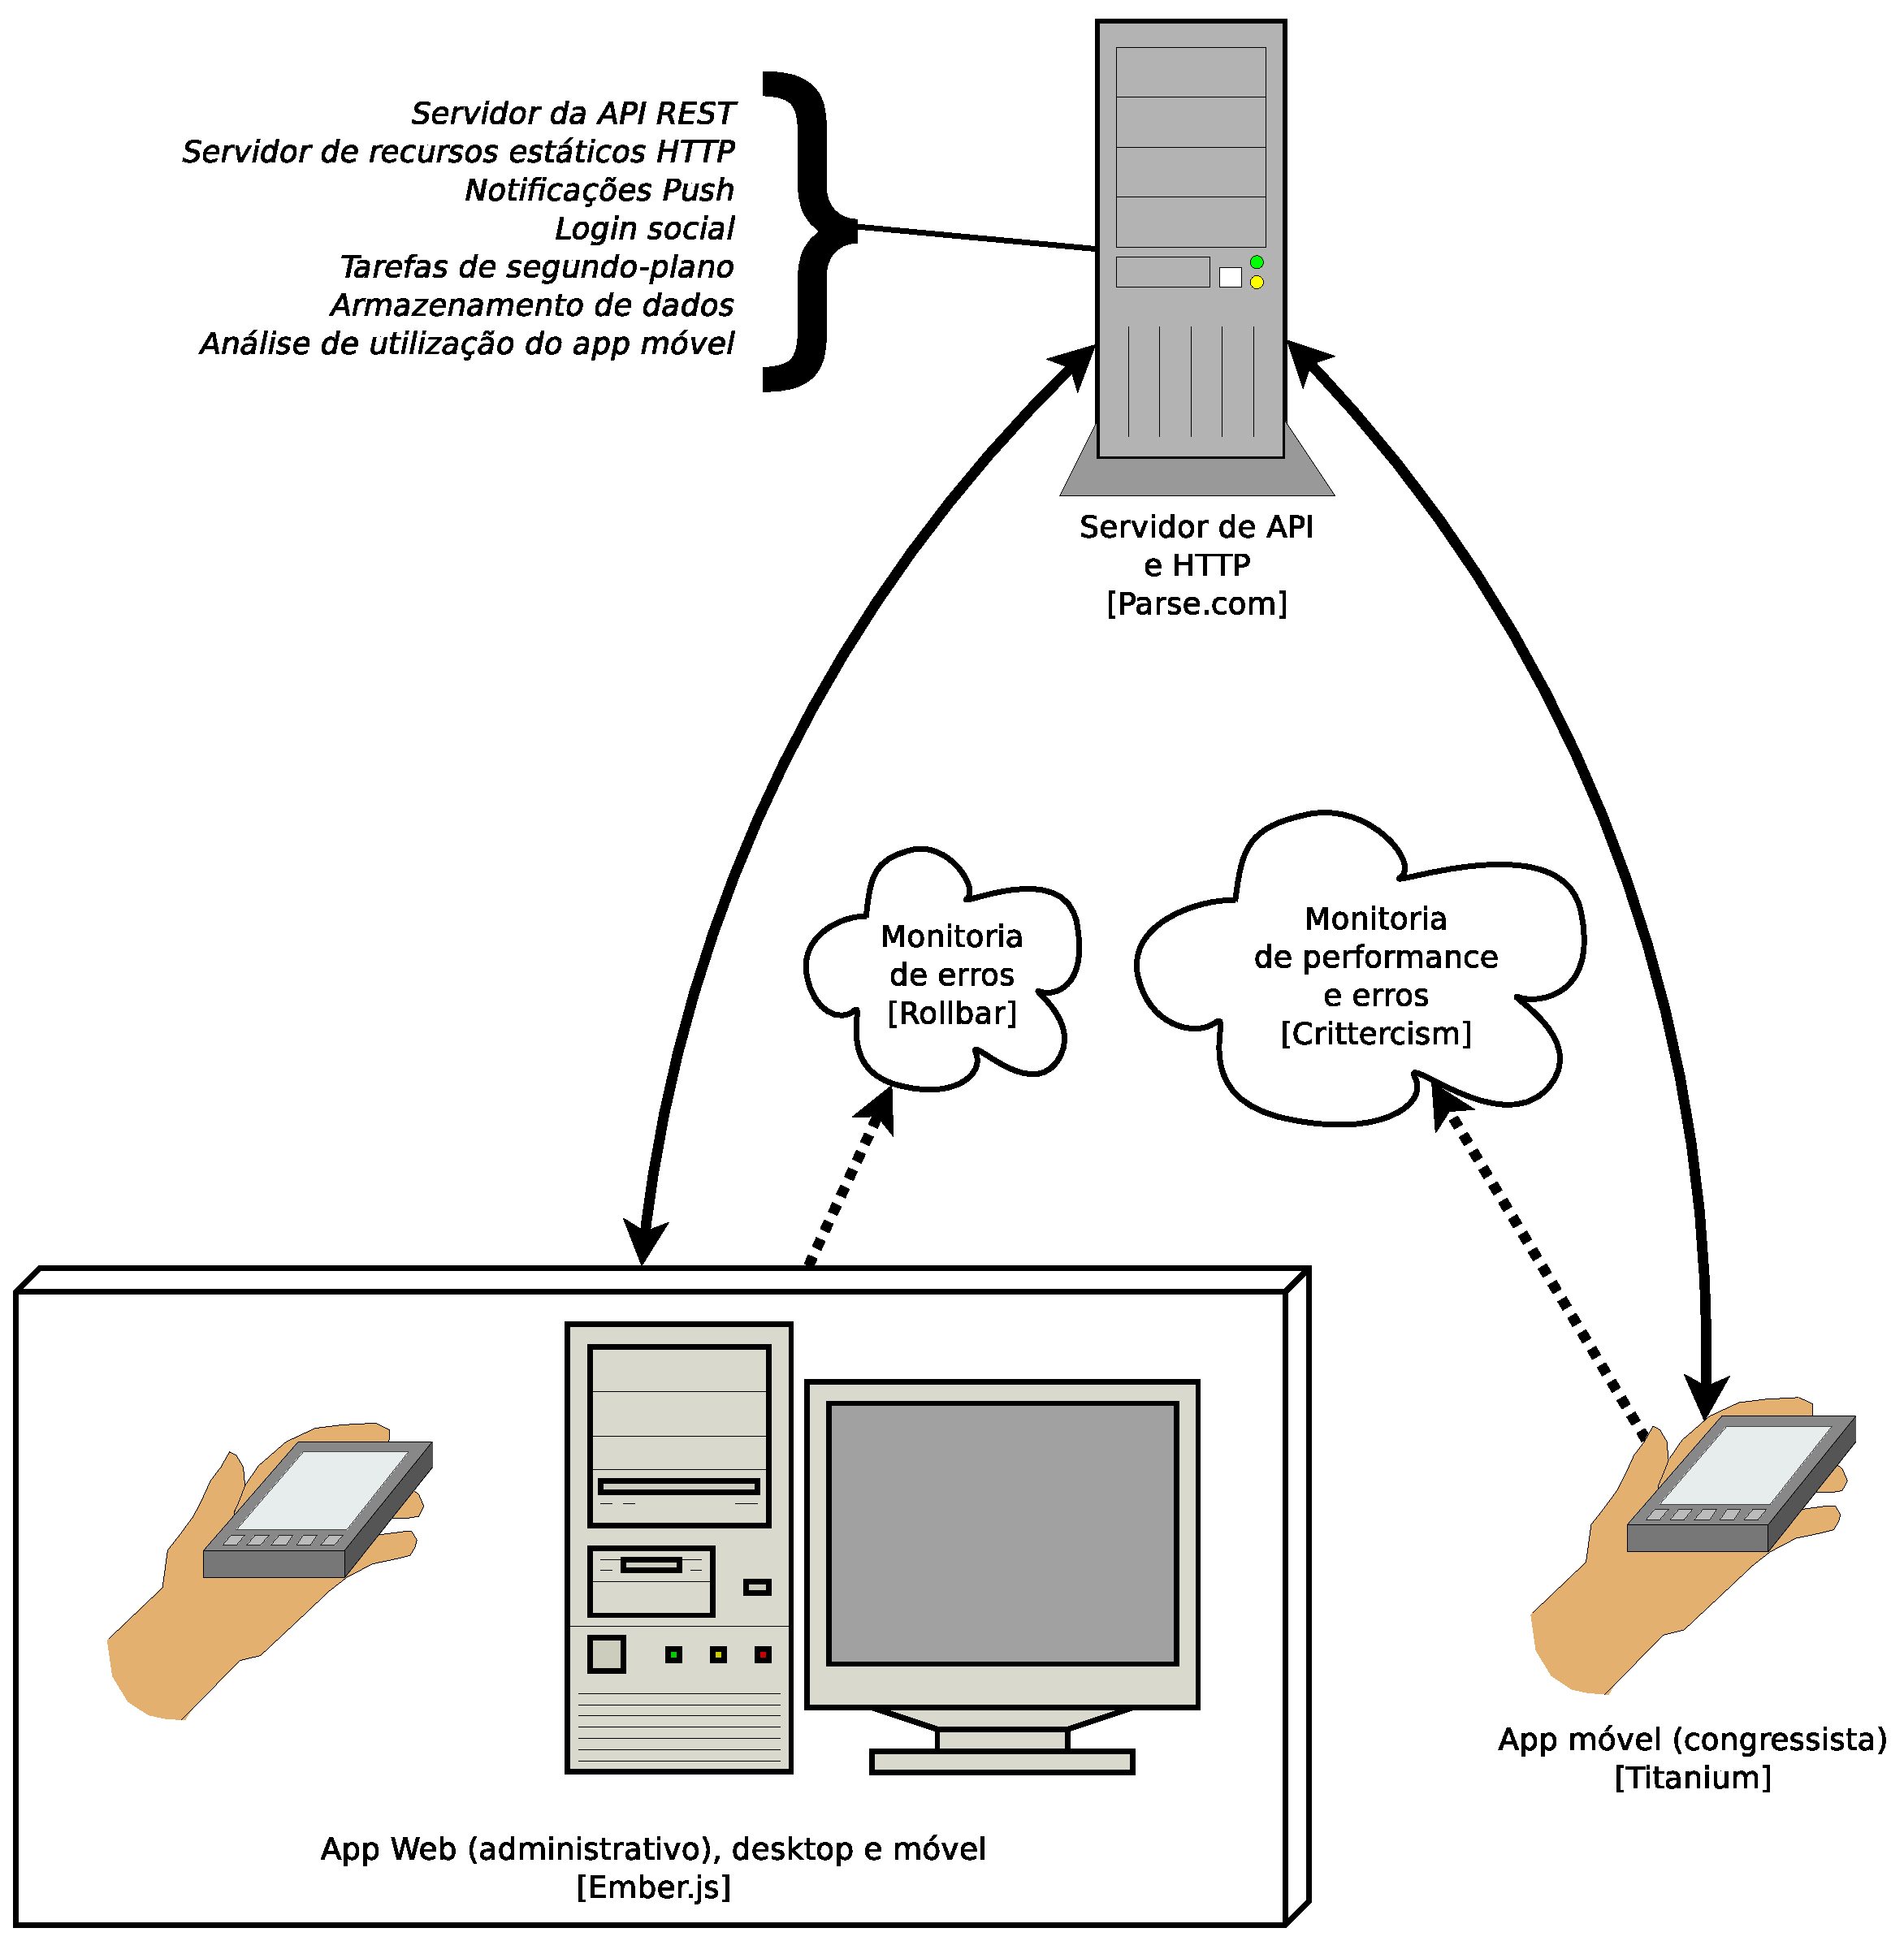
\includegraphics[width=0.8\linewidth]{diagramas/topologia-parse.eps}
	\caption{Diagrama de topologia simples, indicando o uso central dos serviços do Parse}
\end{figure}


%%%%%%%%%%%%%%%%%%%%%%%%%%%%%%%%%%%%%%%%%%%%%%%%%%%%%%%%%%%%%%%%%%%%%%%%%%%%%%%%%%%%%%%%%
\section{Análise do desenvolvimento do sistema}

\subsection{Diagramas de Atividade}

\subsection{Protótipos de telas}

\subsection{Casos de Uso}

\subsubsection*{Usuário - participante}
\subsubsection*{Cliente - organizador}
\subsubsection*{Admin - moderador}

\subsection{Diagramas de Classes}

\subsection{Diagramas de Estado} % vai ser necessário?

\subsection{Diagramas de Sequência} % vai ser necessário?


%%%%%%%%%%%%%%%%%%%%%%%%%%%%%%%%%%%%%%%%%%%%%%%%%%%%%%%%%%%%%%%%%%%%%%%%%%%%%%%%%%%%%%%%%
\postextual
\bibliography{projeto}

\end{document}
